\documentclass[x11names,10pt]{beamer}

\usefonttheme{professionalfonts}

\usepackage[T1]{fontenc}
\usepackage{newpxtext}
\usepackage{newpxmath}
\usepackage{bm}
\usepackage{natbib}
\usepackage[absolute, overlay]{textpos} % showboxes to show boxes.
\usepackage{tikz}
\usepackage{wasysym}

% Fields.
\newcommand*{\Reals}{\mathbb{R}}

% Operators.
\renewcommand*{\O}{\mathcal{O}}
\renewcommand*{\P}{\mathrm{P}}

% Matrices.
\newcommand*{\I}{\mathbf{I}}
\newcommand*{\U}{\mathbf{U}}
\newcommand*{\V}{\mathbf{V}}
\newcommand*{\W}{\mathbf{W}}

% Vectors.
\renewcommand*{\b}{\mathbf{b}}
\renewcommand*{\c}{\mathbf{c}}
\newcommand*{\f}{\mathbf{f}}
\newcommand*{\g}{\mathbf{g}}
\newcommand*{\h}{\mathbf{h}}
\renewcommand*{\o}{\mathbf{o}}
\renewcommand*{\r}{\mathbf{r}}
\newcommand*{\s}{\mathbf{s}}
\newcommand*{\sh}{\hat{\s}}
\newcommand*{\st}{\tilde{\s}}
\newcommand*{\x}{\mathbf{x}}
\newcommand*{\y}{\mathbf{y}}
\newcommand*{\z}{\mathbf{z}}
\newcommand*{\one}{\mathbf{1}}
\newcommand*{\zero}{\mathbf{0}}
\newcommand*{\ETA}{\bm{\eta}}
\newcommand*{\THETA}{\bm{\theta}}
\newcommand*{\PHI}{\bm{\phi}}

% Scalars.
\newcommand*{\tauh}{\hat{\tau}}
\renewcommand*{\th}{\hat{t}}

% LaTeX things.
\renewcommand{\thefootnote}{\fnsymbol{footnote}}

% Other commands.
\newcommand{\bluelink}[2]{\href{#1}{\textcolor{blue}{#2}}}
\newcommand{\blueurl}[1]{\textcolor{blue}{\url{#1}}}

% Make a variant of \vdots without the top vertical space.
\makeatletter
\DeclareRobustCommand{\vvdots}{%
    \vbox{
        \baselineskip4\p@\lineskiplimit\z@
        \kern-\p@
        \hbox{.}\hbox{.}\hbox{.}
    }
}
\makeatother

% Theme settings.
\usetheme{Frankfurt}
\usefonttheme{serif}

% Other Beamer settings.
\setbeamercovered{transparent}
\AtBeginSection[]{%
    \begin{frame}{Outline}
        \tableofcontents[currentsection]
    \end{frame}
}

% Length settings.
% \geometry{papersize={17.0666666666666666667cm, 9.6cm}}
\setlength{\TPHorizModule}{1cm}
\setlength{\TPVertModule}{1cm}

% TikZ commands.
\usetikzlibrary{arrows.meta, positioning}

\tikzstyle{binary} = [
    draw,
    thick,
    circle,
    minimum width=4mm,
    inner sep=0pt,
    fill=green!20
]
\tikzstyle{block} = [minimum width=7mm, minimum height=7mm, thick, rectangle, rounded corners, font=\small, inner sep=2.5pt]
\tikzstyle{cell} = [draw, thick, rounded corners, fill=yellow!20]
\tikzstyle{data} = [draw, block, fill=yellow!20]
\tikzstyle{dense} = [lstm, fill=green!20]
\tikzstyle{filter} = [draw, block, fill=yellow!20]
\tikzstyle{function} = [draw, block, fill=red!20]
\tikzstyle{gate} = [unary, fill=red!20]
\tikzstyle{hmm} = [draw, fill=black!30, circle, minimum width=2mm, inner sep=0pt]
\tikzstyle{label} = [font=\footnotesize]
\tikzstyle{latent} = [draw, block, fill=green!20]
\tikzstyle{layer} = [draw, block, fill=green!20]
\tikzstyle{lstm} = [draw, block, fill=blue!20]
\tikzstyle{path} = [-Latex, thick]
\tikzstyle{plus} = [
    binary,
    append after command={%
        [shorten >= \pgflinewidth, shorten <= \pgflinewidth]
        (\tikzlastnode.north) edge (\tikzlastnode.south)
        (\tikzlastnode.east) edge (\tikzlastnode.west)%
    }
]
\tikzstyle{prod} = [
    binary,
    append after command={%
        node [draw, circle, minimum width=1.5mm, inner sep=0pt]
        at (\tikzlastnode.center) {}%
    }
]
\tikzstyle{state} = [draw, block, fill=blue!20]
\tikzstyle{unary} = [
    draw,
    thick,
    rectangle,
    rounded corners,
    minimum width=7mm,
    minimum height=6mm,
    fill=blue!20
]
\tikzstyle{word} = [text height=1.5ex, text depth=0.25ex]
\tikzstyle{wordmini} = [word, font=\footnotesize, inner sep=0pt]

% Figures.
\graphicspath{{figures/}}

% Title, author, date, classification, etc.
\title{Recurrent neural networks}
\author[Kevin K. Chen]{%
    \texorpdfstring{%
        Kevin K. Chen \\
        \normalsize \bluelink{%
            mailto:kkchen@ccrwest.org%
        }{%
            \texttt{kkchen@ccrwest.org}%
        }%
    }{%
        Kevin K. Chen%
    }%
}
\institute[IDA/CCRL]{Institute for Defense Analyses \\ Center for Communications Research - La Jolla}
\date{February 22, 2018}

% Bibliography commands.
\bibliographystyle{plainnat}
\setcitestyle{round}

\begin{document}

\begin{frame}
    \maketitle
\end{frame}

\begin{frame}{Outline}
    \tableofcontents[
        sectionstyle=show/show,
        subsectionstyle=hide/hide/hide
    ]
\end{frame}

%%% Local Variables:
%%% mode: latex
%%% TeX-master: "../rnn"
%%% End:

\section{Overview}
\subsection{}

\begin{frame}{Resources}
    \begin{itemize}
        \item Ian Goodfellow, Yoshua Bengio, and Aaron Courville.
        \emph{Deep Learning}, ch.~10. MIT Press, 2016
        \nocite{GoodfellowDL}
        \begin{itemize}
            \item Excellent primer
            \item \blueurl{http://www.deeplearningbook.org}
        \end{itemize}
        \item References at the end of these slides
        \item Talk to me! \smiley
    \end{itemize}
\end{frame}

\begin{frame}{Why might I want an RNN?}
    \begin{itemize}
        \item<+-> Universal approximation theorem: dense NNs can model anything nice
        \begin{itemize}
            \item But doesn't specify how hard it is to train
        \end{itemize}
        \item<+-> Silly example: 5 seconds of 44,100 samples/s speech audio $\rightarrow$ 14 transcribed words
        \begin{itemize}
            \item $\exists$ $\sim$3000 commonly-used English words\footnote{The Internet}
            \item $\Reals^{220,500} \to \Reals^{42,000}$ deep dense network?
            \begin{itemize}
                \item Theoretically possible, but please don't
            \end{itemize}
            \item What if I speak 15 words over 5.01~s?
            Must start over!
        \end{itemize}
        \item<+-> More relevant example: predict some quantity from a fluid flow
        \begin{itemize}
            \item Dynamics (e.g., Navier--Stokes) do not change from time $t$ to $t + \Delta t$
            \item Dense network does not know this; allows any dynamical behavior at any $t$
        \end{itemize}
    \end{itemize}
\end{frame}

\begin{frame}{What RNNs do}
    \begin{block}{Key motivation}<+->
        Many processes are sequences through \alert{time} or \alert{steps}, with \alert{time-invariant dynamics}
    \end{block}

    \begin{block}{RNNs are input--output models that impose this structure}<+->
        Interpretation for mechanical/aerospace/electrical engineers: RNNs are \alert{discrete-time nonlinear time-invariant dynamical systems} in which the input/state/output dynamics are learned from (i.e., fitted to) data
    \end{block}

    \begin{itemize}
        \item Note: RNN states usually very difficult to interpret
        \item E.g., RNNs assign same dynamics @ time step 213,913 as 213,914
        \begin{itemize}
            \item Dense NNs treat them entirely separately
        \end{itemize}
        \item Easier to converge to model with ``reasonable''/``desirable'' behavior
        \item Far fewer parameters than naive dense networks
        \item Flexible in how many steps to take
    \end{itemize}
\end{frame}

\begin{frame}{Unfolded computational graphs \& circuit diagrams}
    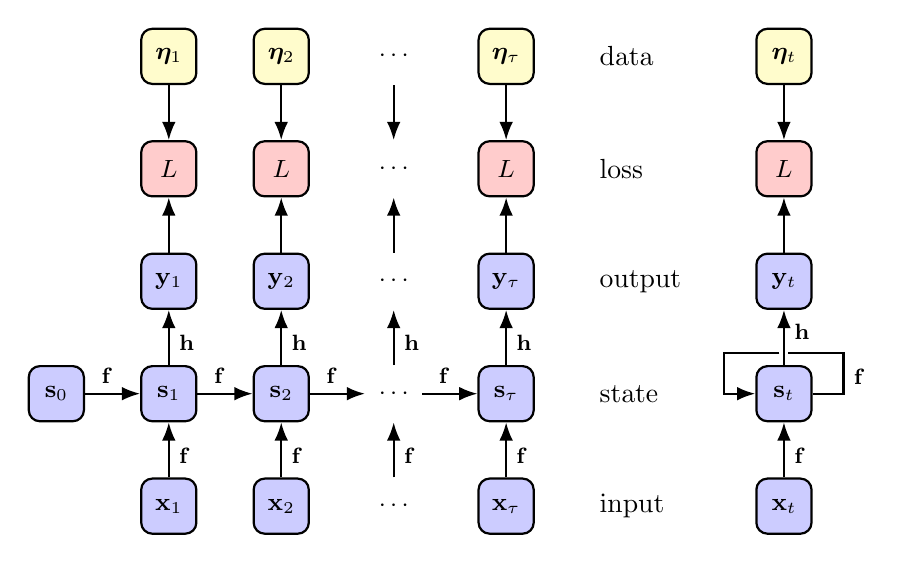
\begin{tikzpicture}[node distance=7mm, auto]
    % Unfolded.

    % States.
    \node (state0) [state] {$\s_0$};
    \node (state1) [state, right=of state0] {$\s_1$};
    \node (state2) [state, right=of state1] {$\s_2$};
    \node (state3) [block, right=of state2] {$\cdots$};
    \node (state4) [state, right=of state3] {$\s_\tau$};

    % Inputs, outputs, losses.
    \foreach\i in {1,2} {
        \node (input\i) [state, below=of state\i] {$\x_\i$};
        \node (output\i) [state, above=of state\i] {$\y_\i$};
        \node (loss\i) [function, above=of output\i] {$L$};
        \node (data\i) [data, above=of loss\i] {$\ETA_\i$};
    }

    \node (input3) [block, below=of state3] {$\cdots$};
    \node (output3) [block, above=of state3] {$\cdots$};
    \node (loss3) [block, above=of output3] {$\cdots$};
    \node (data3) [block, above=of loss3] {$\cdots$};

    \node (input4) [state, below=of state4] {$\x_\tau$};
    \node (output4) [state, above=of state4] {$\y_\tau$};
    \node (loss4) [function, above=of output4] {$L$};
    \node (data4) [data, above=of loss4] {$\ETA_\tau$};

    % Labels.
    \foreach \l in {state, input, output, loss, data} {
        \node [right=of \l4] {\l};
    }

    % Arrows.
    \foreach\i in {1, ..., 4} {
        \draw [path] (input\i) -- node [label, pos=0.4, right] {$\f$} (state\i);
        \draw [path] (state\i) -- node [label, pos=0.4, right] {$\h$} (output\i);
        \draw [path] (output\i) -- (loss\i);
        \draw [path] (data\i) -- (loss\i);
    }

    \foreach\i/\j in {0/1, 1/2, 2/3, 3/4} {
        \draw [path] (state\i) -- node [label, pos=0.4] {$\f$} (state\j);
    }

    % Folded.
    \node (state) [state, right=2.8 cm of state4] {$\s_t$};
    \node (input) [state, below=of state] {$\x_t$};
    \node (output) [state, above=of state] {$\y_t$};
    \node (loss) [function, above=of output] {$L$};
    \node (data) [data, above=of loss] {$\ETA_t$};
    \node (skip) [inner sep=0.5mm, above=1mm of state] {};
    \node (skip l) [coordinate, left=7mm of skip] {};
    \node (skip r) [coordinate, right=7mm of skip] {};

    % Arrows.
    \draw [path] (input) -- node [label, pos=0.4, right] {$\f$} (state);
    \draw [path] (state) -- node [label, pos=0.6, right] {$\h$} (output);
    \draw [path] (output) -- (loss);
    \draw [path] (data) -- (loss);
    \draw [thick] (state) -| node [label, right, pos=0.7] {$\f$} (skip r) -- (skip);
    \draw [path] (skip) -- (skip l) |- (state);
\end{tikzpicture}
%%% Local Variables:
%%% mode: latex
%%% TeX-master: "../rnn"
%%% End:

\end{frame}

\begin{frame}{Recurrent neural networks in one slide}
    \begin{itemize}[<+->]
        \item Express in terms of discrete-time dynamical systems: $t = 0, 1, \dots, \tau$
        \item $\s_t \in \Reals^n$: (cell) state; initial condition $\s_0$ (often $\zero$)
        \item<.-> $\x_t \in \Reals^q$: inputs
        \item $\f: \Reals^n \times \Reals^q \to \Reals^n$: state update
        \item<.-> $\THETA \in \Reals^m$: parameters for $\f$
        \item State update:
        \begin{equation*}
            \s_t = \f(\s_{t-1}, \x_t; \THETA),
            \quad \text{e.g.}, \,
            \s_t = \tanh(\W \s_{t-1} + \U \x_t + \b), \;
            \THETA = (\W, \U, \b)
        \end{equation*}
        \item Outputs: $\y_t \in \Reals^p$, $\h: \Reals^n \to \Reals^p$, parameters $\PHI \in \Reals^l$:
        \begin{equation*}
            \y_t = \h(\s_t; \PHI),
            \quad \text{e.g.}, \,
            \y_t = \mathrm{softmax}(\V \s_{t} + \c), \;
            \PHI = (\V, \c)
        \end{equation*}
        \item That's it!  Now pick $\THETA$ and $\PHI$ to minimize
        \begin{equation*}
            \mathrm{loss} = L(
                \underbrace{(\ETA_1, \dots, \ETA_\tau)}_\text{data},
                \underbrace{(\y_1, \dots, \y_\tau)}_\text{prediction}
            )
        \end{equation*}
    \end{itemize}
\end{frame}

\begin{frame}{Backpropagation through time \& unrolling}
    \begin{itemize}
        \item<+-> I won't bore you with backprop equations; see \href{http://www.deeplearningbook.org}{\textcolor{blue}{Goodfellow's book}}
        \item<.-> It's just a normal gradient via chain rule; any optimizer can be used
        \item<+-> Need to forward and backprop through input--state--output relations, \emph{and} through time
        \begin{itemize}
            \item Forward and backprop generally serial through time
        \end{itemize}
        \item<.-> For state $\in \Reals^n$, inputs $\in \Reals^q$, outputs $\in \Reals^p$, length $\tau$:
        \begin{itemize}
            \item Backprop cost = $\O(\tau n^2) + \O(\tau n p) + \O(\tau n q)$ products
            \item Watch out for very large \# time steps and input/state/output sizes
        \end{itemize}
        \item<+-> Software typically allows you to \alert{unroll} an RNN
        \begin{itemize}
            \item Precomputes entire unfolded computational graph \& all gradients through all time steps
            \item Faster, but more memory consumption
            \item Good for small, fixed-length RNNs
        \end{itemize}
    \end{itemize}
\end{frame}

%%% Local Variables:
%%% mode: latex
%%% TeX-master: "../rnn"
%%% End:

\section{Recurrent neural network connections}
\subsection{}

\begin{frame}{State-to-state connections}
    \begin{columns}
        \begin{column}{0.71\textwidth}
            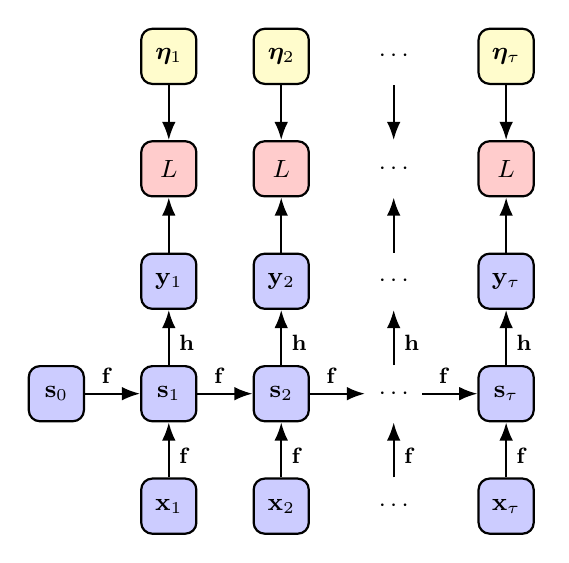
\begin{tikzpicture}[node distance=7mm, auto]
    % States.
    \node (state0) [state] {$\s_0$};
    \node (state1) [state, right=of state0] {$\s_1$};
    \node (state2) [state, right=of state1] {$\s_2$};
    \node (state3) [block, right=of state2] {$\cdots$};
    \node (state4) [state, right=of state3] {$\s_\tau$};

    % Inputs, outputs, losses.
    \foreach\i in {1,2} {
        \node (input\i) [state, below=of state\i] {$\x_\i$};
        \node (output\i) [state, above=of state\i] {$\y_\i$};
        \node (loss\i) [function, above=of output\i] {$L$};
        \node (data\i) [data, above=of loss\i] {$\ETA_\i$};
    }

    \node (input3) [block, below=of state3] {$\cdots$};
    \node (output3) [block, above=of state3] {$\cdots$};
    \node (loss3) [block, above=of output3] {$\cdots$};
    \node (data3) [block, above=of loss3] {$\cdots$};

    \node (input4) [state, below=of state4] {$\x_\tau$};
    \node (output4) [state, above=of state4] {$\y_\tau$};
    \node (loss4) [function, above=of output4] {$L$};
    \node (data4) [data, above=of loss4] {$\ETA_\tau$};

    % Arrows.
    \foreach\i in {1, ..., 4} {
        \draw [path] (input\i) -- node [label, pos=0.4, right] {$\f$} (state\i);
        \draw [path] (state\i) -- node [label, pos=0.4, right] {$\h$} (output\i);
        \draw [path] (output\i) -- (loss\i);
        \draw [path] (data\i) -- (loss\i);
    }

    \foreach\i/\j in {0/1, 1/2, 2/3, 3/4} {
        \draw [path] (state\i) -- node [label, pos=0.4] {$\f$} (state\j);
    }
\end{tikzpicture}
%%% Local Variables:
%%% mode: latex
%%% TeX-master: "../rnn"
%%% End:

            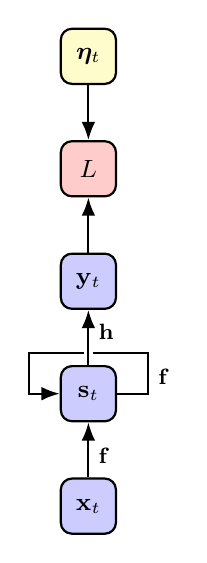
\begin{tikzpicture}[node distance=7mm, auto]
    \node (state) [state] {$\s_t$};
    \node (input) [state, below=of state] {$\x_t$};
    \node (output) [state, above=of state] {$\y_t$};
    \node (loss) [function, above=of output] {$L$};
    \node (data) [data, above=of loss] {$\ETA_t$};
    \node (skip) [inner sep=0.5mm, above=1mm of state] {};
    \node (skip l) [coordinate, left=7mm of skip] {};
    \node (skip r) [coordinate, right=7mm of skip] {};

    % Arrows.
    \draw [path] (input) -- node [label, pos=0.4, right] {$\f$} (state);
    \draw [path] (state) -- node [label, pos=0.6, right] {$\h$} (output);
    \draw [path] (output) -- (loss);
    \draw [path] (data) -- (loss);
    \draw [thick] (state) -| node [label, right, pos=0.7] {$\f$} (skip r) -- (skip);
    \draw [path] (skip) -- (skip l) |- (state);
\end{tikzpicture}
%%% Local Variables:
%%% mode: latex
%%% TeX-master: "../rnn"
%%% End:

        \end{column}
        \begin{column}{0.29\textwidth}
            \begin{itemize}
                \item State-to-state connections are advantageous
                \item Hidden state $\s_t$ (ideally) encodes all information about dynamics up to time $t$, in relatively unconstrained way
                \item Problem: $\s_t$ time-coupling $\implies$ non-parallelizable
            \end{itemize}
        \end{column}
    \end{columns}
\end{frame}

\begin{frame}{Output-to-state connections}
    \begin{columns}
        \begin{column}{0.71\textwidth}
            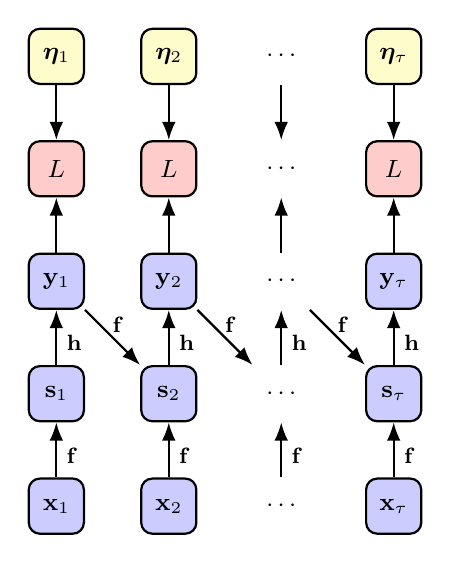
\begin{tikzpicture}[node distance=7mm, auto]
    % States.
    \node (state1) [state] {$\s_1$};
    \node (state2) [state, right=of state1] {$\s_2$};
    \node (state3) [block, right=of state2] {$\cdots$};
    \node (state4) [state, right=of state3] {$\s_\tau$};

    % Inputs, outputs, losses.
    \foreach\i in {1,2} {
        \node (input\i) [state, below=of state\i] {$\x_\i$};
        \node (output\i) [state, above=of state\i] {$\y_\i$};
        \node (loss\i) [function, above=of output\i] {$L$};
        \node (data\i) [data, above=of loss\i] {$\ETA_\i$};
    }

    \node (input3) [block, below=of state3] {$\cdots$};
    \node (output3) [block, above=of state3] {$\cdots$};
    \node (loss3) [block, above=of output3] {$\cdots$};
    \node (data3) [block, above=of loss3] {$\cdots$};

    \node (input4) [state, below=of state4] {$\x_\tau$};
    \node (output4) [state, above=of state4] {$\y_\tau$};
    \node (loss4) [function, above=of output4] {$L$};
    \node (data4) [data, above=of loss4] {$\ETA_\tau$};

    % Arrows.
    \foreach\i in {1, ..., 4} {
        \draw [path] (input\i) -- node [label, pos=0.4, right] {$\f$} (state\i);
        \draw [path] (state\i) -- node [label, pos=0.4, right] {$\h$} (output\i);
        \draw [path] (output\i) -- (loss\i);
        \draw [path] (data\i) -- (loss\i);
    }

    \foreach\i/\j in {1/2, 2/3, 3/4} {
        \draw [path] (output\i) -- node [label, pos=0.6, above] {$\f$} (state\j);
    }
\end{tikzpicture}
%%% Local Variables:
%%% mode: latex
%%% TeX-master: "../rnn"
%%% End:

            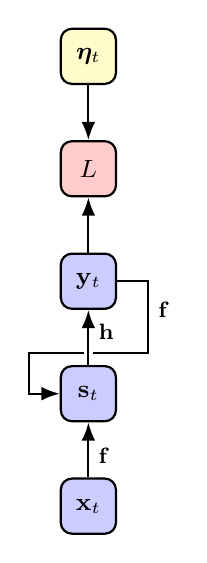
\begin{tikzpicture}[node distance=7mm, auto]
    \node (state) [state] {$\s_t$};
    \node (input) [state, below=of state] {$\x_t$};
    \node (output) [state, above=of state] {$\y_t$};
    \node (loss) [function, above=of output] {$L$};
    \node (data) [data, above=of loss] {$\ETA_t$};
    \node (skip) [inner sep=0.5mm, above=1mm of state] {};
    \node (skip l) [coordinate, left=7mm of skip] {};
    \node (skip r) [coordinate, right=7mm of skip] {};

    % Arrows.
    \draw [path] (input) -- node [label, pos=0.4, right] {$\f$} (state);
    \draw [path] (state) -- node [label, pos=0.6, right] {$\h$} (output);
    \draw [path] (output) -- (loss);
    \draw [path] (data) -- (loss);
    \draw [thick] (output) -| node [label, right, pos=0.7] {$\f$} (skip r) -- (skip);
    \draw [path] (skip) -- (skip l) |- (state);
\end{tikzpicture}
%%% Local Variables:
%%% mode: latex
%%% TeX-master: "../rnn"
%%% End:

        \end{column}
        \begin{column}{0.29\textwidth}
            \begin{itemize}
                \item Weaker: $\y_t$ must encode transition to $\s_{t+1}$ \emph{and} match $\ETA_t$
                \item Forward-prop still non-parallelizable
                \item $\s_t$ not time-coupled
                \item Each time step can be trained independently $\implies$ backprop parallelizable
                \item Not obvious---rederive backprop equations yourself \smiley
            \end{itemize}
        \end{column}
    \end{columns}
\end{frame}

\begin{frame}{Teacher forcing}
    \begin{columns}
        \begin{column}{0.71\textwidth}
            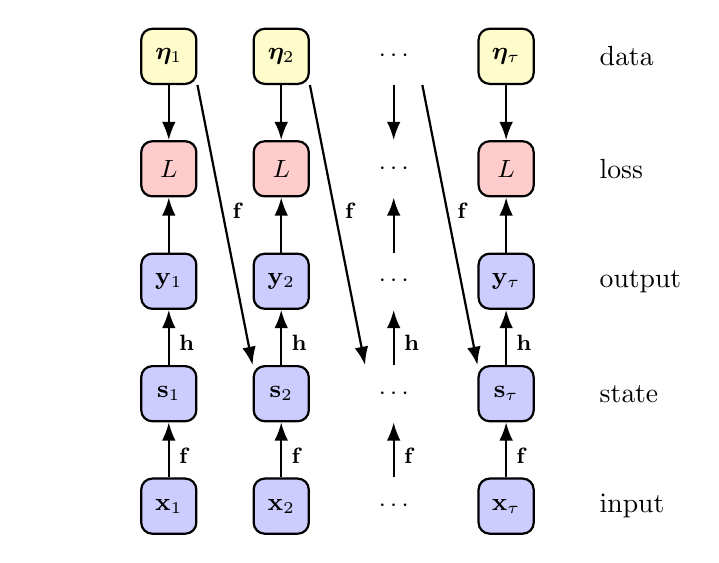
\begin{tikzpicture}[node distance=7mm, auto]
    % States.
    \node (state0) [draw, block, white] {};
    \node (state1) [state, right=of state0] {$\s_1$};
    \node (state2) [state, right=of state1] {$\s_2$};
    \node (state3) [block, right=of state2] {$\cdots$};
    \node (state4) [state, right=of state3] {$\s_\tau$};

    % Inputs, outputs, losses.
    \foreach\i in {1,2} {
        \node (input\i) [state, below=of state\i] {$\x_\i$};
        \node (output\i) [state, above=of state\i] {$\y_\i$};
        \node (loss\i) [function, above=of output\i] {$L$};
        \node (data\i) [data, above=of loss\i] {$\ETA_\i$};
    }

    \node (input3) [block, below=of state3] {$\cdots$};
    \node (output3) [block, above=of state3] {$\cdots$};
    \node (loss3) [block, above=of output3] {$\cdots$};
    \node (data3) [block, above=of loss3] {$\cdots$};

    \node (input4) [state, below=of state4] {$\x_\tau$};
    \node (output4) [state, above=of state4] {$\y_\tau$};
    \node (loss4) [function, above=of output4] {$L$};
    \node (data4) [data, above=of loss4] {$\ETA_\tau$};

    % Labels.
    \foreach \l in {state, input, output, loss, data} {
        \node [right=of \l4] {\l};
    }

    % Arrows.
    \foreach\i in {1, ..., 4} {
        \draw [path] (input\i) -- node [label, pos=0.4, right] {$\f$} (state\i);
        \draw [path] (state\i) -- node [label, pos=0.4, right] {$\h$} (output\i);
        \draw [path] (output\i) -- (loss\i);
        \draw [path] (data\i) -- (loss\i);
    }

    \foreach\i/\j in {1/2, 2/3, 3/4} {
        \draw [path] (data\i.-45) -- node [label, pos=0.45, right] {$\f$} (state\j.135);
    }
\end{tikzpicture}
%%% Local Variables:
%%% mode: latex
%%% TeX-master: "../rnn"
%%% End:

            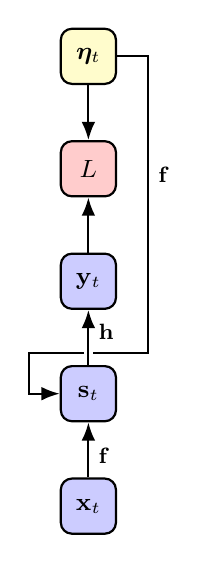
\begin{tikzpicture}[node distance=7mm, auto]
    \node (state) [state] {$\s_t$};
    \node (input) [state, below=of state] {$\x_t$};
    \node (output) [state, above=of state] {$\y_t$};
    \node (loss) [function, above=of output] {$L$};
    \node (data) [data, above=of loss] {$\ETA_t$};
    \node (skip) [inner sep=0.5mm, above=1mm of state] {};
    \node (skip l) [coordinate, left=7mm of skip] {};
    \node (skip r) [coordinate, right=7mm of skip] {};

    % Arrows.
    \draw [path] (input) -- node [label, pos=0.4, right] {$\f$} (state);
    \draw [path] (state) -- node [label, pos=0.6, right] {$\h$} (output);
    \draw [path] (output) -- (loss);
    \draw [path] (data) -- (loss);
    \draw [thick] (data) -| node [label, right, pos=0.7] {$\f$} (skip r) -- (skip);
    \draw [path] (skip) -- (skip l) |- (state);
\end{tikzpicture}
%%% Local Variables:
%%% mode: latex
%%% TeX-master: "../rnn"
%%% End:

        \end{column}
        \begin{column}{0.29\textwidth}
            \begin{itemize}
                \item Training: use data point $\ETA_{t-1}$ for $\s_t$
                \item Forward \& backprop parallelizable
                \item Inference: use architecture on previous slide (minus $\ETA_t$ and $L$)
                \item Can be combined with state-to-state or output-to-state connections for better performance
            \end{itemize}
        \end{column}
    \end{columns}
\end{frame}

\begin{frame}{Long short-term memory, figure}
    \begin{center}
        \vspace{-4mm}
        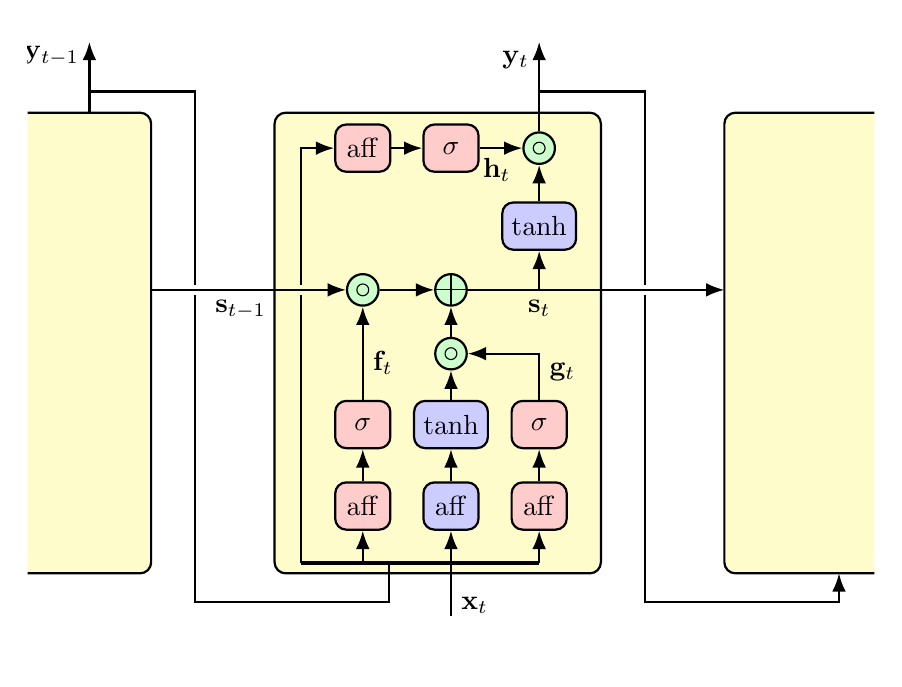
\begin{tikzpicture}[node distance=1cm, x=1.12cm, y=9mm, auto]
    \clip (-4.8, 3.7) rectangle (4.8, -5.2);

    % Cells.
    \draw [cell] (-7.1, 2.5) rectangle (-3.4, -4.0);
    \draw [cell] (-2, 2.5) rectangle (1.7, -4.0);
    \draw [cell] (3.1, 2.5) rectangle (6.8, -4.0);

    % Nodes.
    \node (input) [coordinate] at (0, -4.6) {};
    \node (prev output) [coordinate] at (-4.1, 3.5) {};

    \node (plus) [plus] at (0, 0) {};

    \node (forget prod) [prod] at (-1, 0) {};
    \node (forget sigmoid) [gate] at (-1, -1.9) {$\sigma$};
    \node (forget affine) [gate] at (-1, -3.05) {$\mathrm{aff}$};

    \node (input prod) [prod] at (0, -0.9) {};
    \node (input sigmoid) [gate] at (1, -1.9) {$\sigma$};
    \node (input affine) [gate] at (1, -3.05) {$\mathrm{aff}$};
    \node (input tanh) [unary] at (0, -1.9) {$\tanh$};
    \node (input tanh affine) [unary] at (0, -3.05) {$\mathrm{aff}$};

    \node (state) [coordinate] at (1, 0) {};

    \node (output tanh) [unary] at (1, 0.9) {$\tanh$};
    \node (output prod) [prod] at (1, 2) {};
    \node (output sigmoid) [gate] at (0, 2) {$\sigma$};
    \node (output affine) [gate] at (-1, 2) {$\mathrm{aff}$};
    \node (output) [coordinate] at (1, 3.5) {};

    % Paths.

    % Inputs.
    \draw [path] (-4.1, 2.5) -- node [left, pos=0.8] {$\y_{t-1}$} (prev output);
    \draw [thick] (-4.1, 2.8) -| (-2.9, 0.075);
    \draw [thick] (-2.9, -0.075) |- (-0.7, -4.4) -- (-0.7, -3.85);
    \draw [thick] (input) -- node [right, pos=0.2] {$\x_t$} (0, -3.85);
    \draw [path] (-3.4, 0) -- node [pos=0.46, below] {$\s_{t-1}$} (forget prod);

    % Internal stuff.
    \draw [path] (forget affine) -- (forget sigmoid);
    \draw [path] (forget sigmoid) -- node [right, pos=0.4] {$\f_t$} (forget prod);
    \draw [path] (forget prod) -- (plus);

    \draw [path] (input affine) -- (input sigmoid);
    \draw [path] (input sigmoid) |- node [right, pos=0.3] {$\g_t$} (input prod);
    \draw [path] (input prod) -- (plus);

    \draw [path] (input tanh affine) -- (input tanh);
    \draw [path] (input tanh) -- (input prod);

    \draw [path] (plus) -- (3.1, 0);
    \draw [path] (state) -- node [pos=0, below] {$\s_t$} (output tanh);

    \draw [path] (output tanh) -- (output prod);
    \draw [path] (output affine) -- (output sigmoid);
    \draw [path] (output sigmoid) -- node [pos=0.4, below] {$\h_t$} (output prod);

    % Input to affine paths.
    \draw [ultra thick] (-1.7, -3.85) -- (1, -3.85);
    \draw [path] (-1, -3.85) -- (forget affine);
    \draw [path] (0, -3.85) -- (input tanh affine);
    \draw [path] (1, -3.85) -- (input affine);
    \draw [thick] (-1.7, -3.85) -- (-1.7, -0.075);
    \draw [path] (-1.7, 0.075) |- (output affine);

    % Outputs.
    \draw [path] (output prod) -- node [left, pos=0.8] {$\y_t$} (output);
    \draw [thick] (1, 2.8) -| (2.2, 0.075);
    \draw [path] (2.2, -0.075) |- (4.4, -4.4) -- (4.4, -4);
\end{tikzpicture}

%%% Local Variables:
%%% mode: latex
%%% TeX-master: "../rnn"
%%% End:

        \vspace{-7mm}
    \end{center}
\end{frame}

\begin{frame}{Long short-term memory, equations}
    \begin{itemize}
        \item<+-> Inputs: $\x_t \in \Reals^q$; cell state: $\s_t \in \Reals^n$; output: $\y_t \in (-1, 1)^n$
        \item<.-> Weights and biases: $\U \in \Reals^{n \times q}$, $\W \in \Reals^{n \times n}$, $\b \in \Reals^n$
        \item<.-> $\sigma(x) = 1 / (1 + e^{-x})$, element-wise
        \item<.-> $\circ$: element-wise product
        \item<+-> Gates:
        \begin{align*}
            \text{forget:} \quad \f_t &= \sigma(\U_\f \x_t + \W_\f \y_{t-1} + \b_\f) \in (0, 1)^n \\
            \text{input:} \quad \g_t &= \sigma(\U_\g \x_t + \W_\g \y_{t-1} + \b_\g) \in (0, 1)^n \\
            \text{output:} \quad \h_t &= \sigma(\U_\h \x_t + \W_\h \y_{t-1} + \b_\h) \in (0, 1)^n
        \end{align*}
        \item<+-> Dynamics:
        \begin{align*}
            \text{state update:} \quad \s_t &= \f_t \circ \s_{t-1} + \g_t \circ \tanh(\U_\s \x_t + \W_\s \y_{t-1} + \b_\s) \\
            \text{output:} \quad \y_t &= \h_t \circ \tanh(\s_t)
        \end{align*}
        \item<.-> Total: $4 n (n + q + 1)$ parameters
    \end{itemize}
\end{frame}

\begin{frame}{Long short-term memory, comments}
    \begin{block}{}
        \vspace{-5mm}
        \begin{align*}
            \text{state update:} \quad \s_t &= \alert<2->{\f_t} \circ \s_{t-1} + \g_t \circ \tanh(\U_\s \x_t + \W_\s \y_{t-1} + \b_\s) \\
            \text{output:} \quad \y_t &= \h_t \circ \tanh(\s_t)
        \end{align*}
    \end{block}

    \begin{itemize}
        \item<+-> Introduced by~\citet{HochreiterNC97}; analysis by \citet{GreffIEEENNLS17}
        \item<.-> \rnn{} problem: long backprop through time leads to vanishing/exploding gradients
        \item<+-> Key insight: \alert{forget gate $\f_t$} reduces dependency on states far in the past $\implies$ better-behaved gradients
        \item<.-> Gating behavior determined by inputs/outputs, rather than statically
        \item<+-> Typically initialize forget bias to $\b_\f = \one$~\citep{GersNC00,JozefowiczICML15}
        \begin{itemize}
            \item Otherwise, \lstm{} will forget too aggressively early in training
        \end{itemize}
        \item<.-> Can include state $\s_t$ in gate operands (peephole connections)
        \item<+-> The most common and arguably the strongest \rnn{} architecture in use today \citep{JozefowiczICML15}
    \end{itemize}
\end{frame}

\begin{frame}{Gated recurrent unit, figure}
    \begin{center}
        \vspace{-7mm}
        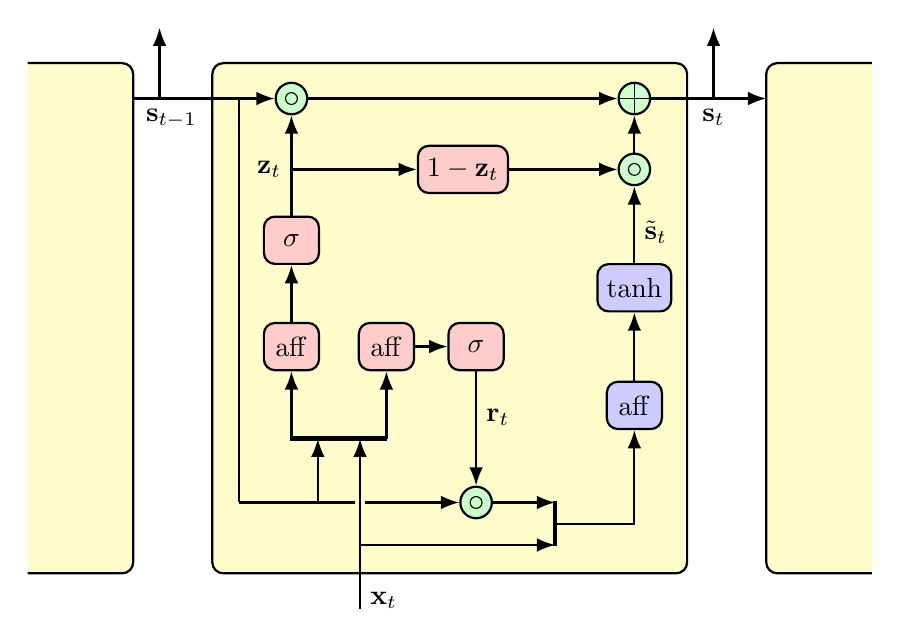
\begin{tikzpicture}[node distance=1cm, x=6.7mm, y=9mm, auto]
    \clip (-6, -0.2) rectangle (10, 8);

    % Cells.
    \draw [cell] (-12, 0.3) rectangle (-4, 7.5);
    \draw [cell] (-2.5, 0.3) rectangle (6.5, 7.5);
    \draw [cell] (8, 0.3) rectangle (15, 7.5);

    % Nodes.
    \node (input) [coordinate] at (0.3, -0.2) {};

    \node (update affine) [gate] at (-1, 3.5) {$\mathrm{aff}$};
    \node (update sigmoid) [gate] at (-1, 5) {$\sigma$};

    \node (reset affine) [gate] at (0.8, 3.5) {$\mathrm{aff}$};
    \node (reset sigmoid) [gate] at (2.5, 3.5) {$\sigma$};

    \node (state prod) [prod] at (-1, 7) {};
    \node (update prod) [prod] at (2.5, 1.3) {};

    \node (prev state) [coordinate] at (-4, 7) {};
    \node (prev state 0) [coordinate] at (-2, 7) {};
    \node (prev state 1) [coordinate] at (-2, 1.3) {};

    \node (subtract) [gate] at (2.25, 6) {$1 - \z_t$};
    \node (alt prod) [prod] at (5.5, 6) {};

    \node (alt affine) [unary] at (5.5, 2.67) {$\mathrm{aff}$};
    \node (alt tanh) [unary] at (5.5, 4.33) {$\tanh$};

    \node (sum) [plus] at (5.5, 7) {};
    \node (state) [coordinate] at (8, 7) {};

    % Paths.
    \draw [path] (input) -- node [right, pos=0.05] {$\x_t$} (0.3, 2.2);

    \draw [ultra thick] (-1.02, 2.2) -- (0.82, 2.2);
    \draw [path] (-1, 2.2) -- (update affine);
    \draw [path] (0.8, 2.2) -- (reset affine);

    \draw [path] (update affine) -- (update sigmoid);
    \draw [path] (reset affine) -- (reset sigmoid);

    \draw [path] (prev state) -- node [below, pos=0.27] {$\s_{t-1}$} (state prod);
    \draw [path] (-3.5, 7) -- (-3.5, 8);
    \draw [path] (update sigmoid) -- (state prod);
    \draw [path] (-1, 6) -- node [left, pos=0] {$\z_t$}(subtract);
    \draw [path] (subtract) -- (alt prod);
    \draw [path] (state prod) -- (sum);
    \draw [path] (reset sigmoid) -- node [right, pos=0.4] {$\r_t$} (update prod);

    \draw [thick] (prev state 0) -- (prev state 1);
    \draw [thick] (prev state 1) -- (0.2, 1.3);
    \draw [path] (0.4, 1.3) -- (update prod);
    \draw [path] (-0.5, 1.3) -- (-0.5, 2.2);

    \draw [ultra thick] (4, 1.32) -- (4, 0.68);
    \draw [path] (update prod) -- (4, 1.3);
    \draw [path] (0.3, 0.7) -- (4, 0.7);
    \draw [path] (4, 1) -| (alt affine);
    \draw [path] (alt affine) -- (alt tanh);
    \draw [path] (alt tanh) -- node [right, pos=0.4] {$\st_t$} (alt prod);
    \draw [path] (alt prod) -- (sum);

    \draw [path] (sum) -- (state);
    \draw [path] (7, 7) -- node [below, pos=0] {$\s_t$}(7, 8);
\end{tikzpicture}

%%% Local Variables:
%%% mode: latex
%%% TeX-master: "../rnn"
%%% End:

        \vspace{-7mm}
    \end{center}
\end{frame}

\begin{frame}{Gated recurrent unit, equations}
    \begin{itemize}
        \item<+-> Inputs: $\x_t \in \Reals^q$; cell state and output: $\s_t \in (-1, 1)^n$
        \item<.-> Weights and biases: $\U \in \Reals^{n \times q}$, $\W \in \Reals^{n \times n}$, $\b \in \Reals^n$
        \item<+-> Gates:
        \begin{align*}
            \text{reset:} \quad \r_t &= \sigma(\U_\r \x_t + \W_\r \s_{t-1} + \b_\r) \in (0, 1)^n \\
            \text{update:} \quad \z_t &= \sigma(\U_\z \x_t + \W_\z \s_{t-1} + \b_\z) \in (0, 1)^n
        \end{align*}
        \item<+-> Dynamics:
        \begin{align*}
            \text{alternate state:} \quad \st_t &= \tanh(\U_\s \x_t + \W_\s (\r_t \circ \s_{t-1}) + \b_\s) \in (-1, 1)^n \\
            \text{state update:} \quad \s_t &= \z_t \circ \s_{t-1} + (\one - \z_t) \circ \st_t
        \end{align*}
        \item<.-> Total: $3 n (n + q + 1)$ parameters
    \end{itemize}
\end{frame}

\begin{frame}{Gate recurrent unit, comments}
    \begin{block}{}
        \vspace{-5mm}
        \begin{align*}
            \text{alternate state:} \quad \st_t &= \tanh(\U_\s \x_t + \W_\s (\alert{\r_t} \circ \s_{t-1}) + \b_\s) \in (-1, 1)^n \\
            \text{state update:} \quad \s_t &= \alert{\z_t} \circ \s_{t-1} + \alert{(\one - \z_t)} \circ \st_t
        \end{align*}
    \end{block}

    \begin{itemize}
        \item<+-> Introduced by \citet{ChoEMNLP14}
        \item<.-> \alert{Reset gate $\r_t$} limits how much $\s_{t-1}$ plays into $\st_t$
        \item<.-> \alert{Update gate $\z_t$} similar to \lstm{} forget gate, but linearly interpolates between $\s_{t-1}$ and $\st_t$
        \item<+-> Hand-wavy argument: \lstm{} output \& output gate not really necessary
        \begin{itemize}
            \item Too flexible, not enough structure, too many parameters $\implies$ harder to train
            \item Recall: \rnn{}s preferable to dense networks because imposing structure makes good network easier to obtain via optimization
        \end{itemize}
        \item<+-> Also arguably the strongest \rnn{} architecture today \citep{JozefowiczICML15}
        \begin{itemize}
            \item No consensus on \lstm{} vs.~\gru{}
        \end{itemize}
    \end{itemize}
\end{frame}

\begin{frame}{Bidirectionality}
    \begin{columns}
        \begin{column}{0.53\textwidth}
            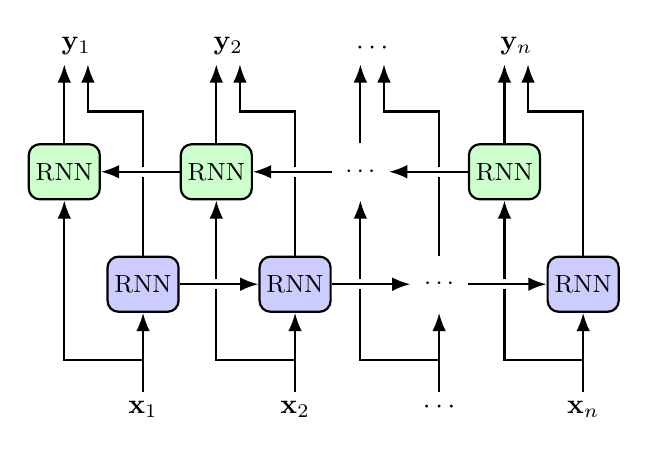
\begin{tikzpicture}[node distance=1cm]
    % Reverse LSTM cells.
    \node (reverse 1) [lstm, fill=green!20] {RNN};
    \node (reverse 2) [lstm, fill=green!20, right=of reverse 1] {RNN};
    \node (reverse 3) [block, right=of reverse 2] {$\cdots$};
    \node (reverse 4) [lstm, fill=green!20, right=of reverse 3] {RNN};

    % Forward LSTM cells.
    \foreach \x in {1, 2, 4} {%
        \node (forward \x) [lstm, below=7mm of reverse \x, xshift=1cm] {RNN};
    }

    \node (forward 3) [block, below=7mm of reverse 3, xshift=1cm] {$\cdots$};

    % Labels.
    \foreach \j in {1, 2} {%
        \node (input \j) [below=of forward \j] {$\x_\j$};
        \node (output \j) [above=of reverse \j, xshift=1.5mm] {$\y_\j$};
    }

    \node (input 3) [below=of forward 3] {$\cdots$};
    \node (input 4) [below=of forward 4] {$\x_n$};
    \node (output 3) [above=of reverse 3, xshift=1.5mm] {$\cdots$};
    \node (output 4) [above=of reverse 4, xshift=1.5mm] {$\y_n$};

    % Coordinates.
    \foreach \j in {1, ..., 4} {%
        \node (i \j) [coordinate, below=6mm of forward \j] {};
        % Corner coordinate.
        \node (y \j) [coordinate, above=4mm of reverse \j, xshift=3mm] {};
        % Two output coordinates.
        \node (forward y \j) [coordinate, above=6mm of y \j] {};
        \node (reverse y \j) [coordinate, above=of reverse \j] {};
    }

    % Coordinates around the reverse state flow.
    \foreach \j in {1, ..., 3} {%
        \node (reverse state down \j) [coordinate, above=10mm of forward \j] {};
        \node (reverse state up \j) [coordinate, above=1.25mm of reverse state down \j] {};
    }

    % Coordinates around the forward state flow.
    \foreach \j in {2, ..., 4} {%
        \node (forward state up \j) [coordinate, below=10mm of reverse \j] {};
        \node (forward state down \j) [coordinate, below=1.25mm of forward state up \j] {};
    }

    % Paths.

    % Cell to cell flow.
    \foreach \j in {1, ..., 3} {
        \pgfmathtruncatemacro{\k}{\j + 1}

        \draw [path] (forward \j) -- (forward \k);
        \draw [path] (reverse \k) -- (reverse \j);
    }

    % Input to forward LSTM and reverse LSTM to output.
    \foreach \j in {1, ..., 4} {%
        \draw [path] (input \j) -- (forward \j);
        \draw [path] (reverse \j) -- (reverse y \j);
    }

    % Secondary input/output paths with no path intersections.
    \draw [path] (i 1) -| (reverse 1);
    \draw [path] (forward 4) |- (y 4) -- (forward y 4);

    % Forward LSTM outputs.
    \foreach \j in {1, ..., 3} {%
        \draw [thick] (forward \j) -- (reverse state down \j);
        \draw [path] (reverse state up \j) |- (y \j) -- (forward y \j);
    }

    % Reverse LSTM inputs.
    \foreach \j in {2, ..., 4} {%
        \draw [thick] (i \j) -| (forward state down \j);
        \draw [path] (forward state up \j) -- (reverse \j);
    }
\end{tikzpicture}

%%% Local Variables:
%%% mode: latex
%%% TeX-master: "../rnn"
%%% End:

        \end{column}
        \begin{column}{0.47\textwidth}
            \begin{itemize}[<.->]
                \item<+-> Humans tend to process sequences begin-to-end
                \item Often, \rnn{}s need not do the same
                \item E.g., English word generation: \texttt{\ldots{}ing} likely followed by \texttt{<end>}, but also \texttt{ng<end>} likely preceded by \texttt{\ldots{}i}
            \end{itemize}
            \uncover<+->{Bidirectional \rnn{}: \textcolor{blue}{forward}- and \textcolor{Green4}{reverse}-directional \rnn{}s with separate states, outputs, weights, biases}
            \begin{itemize}[<.->]
                \item Each receives same inputs
                \item Outputs concatenated at each step
                \item Easy to implement---1 line of code
                \item \citet{SchusterIEEESP97}
            \end{itemize}
        \end{column}
    \end{columns}
\end{frame}

\begin{frame}{Stacked \rnn{}s}
    \begin{columns}
        \begin{column}{0.41\textwidth}
            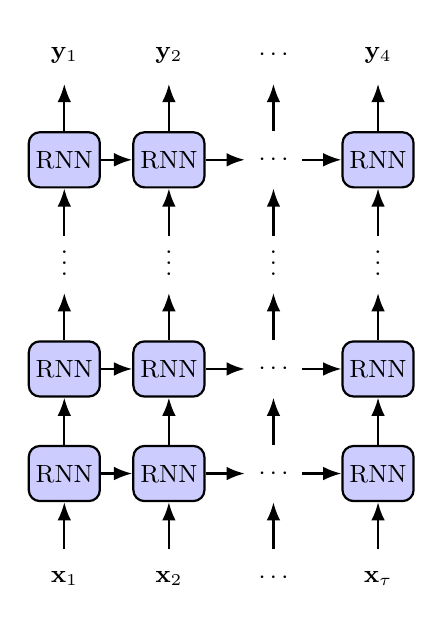
\begin{tikzpicture}[node distance=6mm]
    % Nodes.

    % Inputs.
    \node (node 01) [block] {$\x_1$};
    \node (node 02) [block, right=of node 01] {$\x_2$};
    \node (node 03) [block, right=of node 02] {$\cdots$};
    \node (node 04) [block, right=of node 03] {$\x_\tau$};

    % RNNs.
    \foreach \i in {1, 2, 4} {%
        \node (node 1\i) [lstm, above=of node 0\i] {RNN};
        \node (node 2\i) [lstm, above=of node 1\i] {RNN};
        \node (node 3\i) [block, above=of node 2\i] {\vvdots};
        \node (node 4\i) [lstm, above=of node 3\i] {RNN};
        \node (node 5\i) [block, above=of node 4\i] {$\y_\i$};
    }

    % Ellipses.
    \node (node 13) [block, above=of node 03] {$\cdots$};
    \node (node 23) [block, above=of node 13] {$\cdots$};
    \node (node 33) [block, above=of node 23] {\vvdots};
    \node (node 43) [block, above=of node 33] {$\cdots$};
    \node (node 53) [block, above=of node 43] {$\cdots$};

    % Horizontal arrows.
    \foreach \n in {1, 2, 4} {%
        \foreach \i in {1, ..., 3} {
            \pgfmathtruncatemacro{\j}{\i + 1}
            \draw [path] (node \n\i) -- (node \n\j);
        }
    }

    % Vertical arrows.
    \foreach \n in {0, ..., 4} {
        \pgfmathtruncatemacro{\m}{\n + 1}

        \foreach \i in {1, ..., 4} {%
            \draw [path] (node \n\i) -- (node \m\i);
        }
    }
\end{tikzpicture}%
%%% Local Variables:
%%% mode: latex
%%% TeX-master: "../rnn"
%%% End:

        \end{column}
        \begin{column}{0.59\textwidth}
            \begin{itemize}
                \item \lstm{}s and \gru{}s are powerful, but they're still shallow
                \item By far the most common way to make them deep is to \alert{stack} them
                \item Output of one \rnn{} used as input to another; repeat \emph{ad infinitum}
                \pause
                \item \rnn{}s can be bidirectional
                \item Easy to implement---1 or 2 lines of code
                \item Common to use same state size in all layers
                \begin{itemize}
                    \item I doubt there's much rigorous justification
                \end{itemize}
            \end{itemize}
        \end{column}
    \end{columns}
\end{frame}

\begin{frame}{Other deep \rnn{}s: deep input-to-state connections}
    \hspace{2cm}
    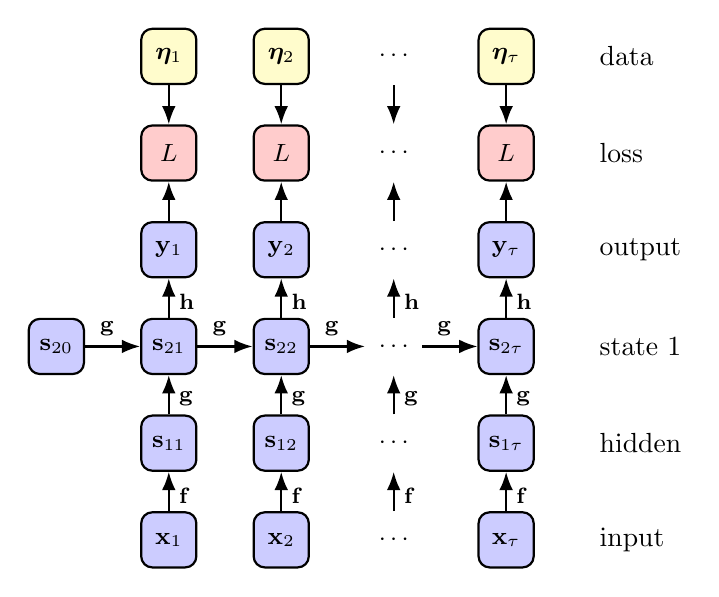
\begin{tikzpicture}[node distance=5mm, auto]
    % States.
    \node (state11) [state] {$\s_{11}$};
    \node (state12) [state, right=7mm of state11] {$\s_{12}$};
    \node (state13) [block, right=7mm of state12] {$\cdots$};
    \node (state14) [state, right=7mm of state13] {$\s_{1\tau}$};

    \node (state21) [state, above=of state11] {$\s_{21}$};
    \node (state20) [state, left=7mm of state21] {$\s_{20}$};
    \node (state22) [state, above=of state12] {$\s_{22}$};
    \node (state23) [block, above=of state13] {$\cdots$};
    \node (state24) [state, above=of state14] {$\s_{2\tau}$};


    % Inputs, outputs, losses.
    \foreach\i in {1,2} {
        \node (input\i) [state, below=of state1\i] {$\x_\i$};
        \node (output\i) [state, above=of state2\i] {$\y_\i$};
        \node (loss\i) [function, above=of output\i] {$L$};
        \node (data\i) [data, above=of loss\i] {$\ETA_\i$};
    }

    \node (input3) [block, below=of state13] {$\cdots$};
    \node (output3) [block, above=of state23] {$\cdots$};
    \node (loss3) [block, above=of output3] {$\cdots$};
    \node (data3) [block, above=of loss3] {$\cdots$};

    \node (input4) [state, below=of state14] {$\x_\tau$};
    \node (output4) [state, above=of state24] {$\y_\tau$};
    \node (loss4) [function, above=of output4] {$L$};
    \node (data4) [data, above=of loss4] {$\ETA_\tau$};

    % Labels.
    \foreach \l in {input, output, loss, data} {
        \node [right=7mm of \l4] {\l};
    }

    \node [right=7mm of state14] {hidden};
    \node [right=7mm of state24] {state 1};

    % Arrows.
    \foreach\i in {1, ..., 4} {
        \draw [path] (input\i) -- node [label, pos=0.4, right] {$\f$} (state1\i);
        \draw [path] (state1\i) -- node [label, pos=0.4, right] {$\g$} (state2\i);
        \draw [path] (state2\i) -- node [label, pos=0.4, right] {$\h$} (output\i);
        \draw [path] (output\i) -- (loss\i);
        \draw [path] (data\i) -- (loss\i);
    }

    \foreach\i/\j in {0/1, 1/2, 2/3, 3/4} {
        \draw [path] (state2\i) -- node [label, pos=0.4] {$\g$} (state2\j);
    }
\end{tikzpicture}
%%% Local Variables:
%%% mode: latex
%%% TeX-master: "../rnn"
%%% End:

    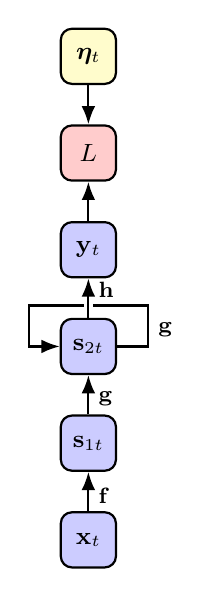
\begin{tikzpicture}[node distance=5mm, auto]
    \node (state 1) [state] {$\s_{1t}$};
    \node (state 2) [state, above=of state 1] {$\s_{2t}$};
    \node (input) [state, below=of state 1] {$\x_t$};
    \node (output) [state, above=of state 2] {$\y_t$};
    \node (loss) [function, above=of output] {$L$};
    \node (data) [data, above=of loss] {$\ETA_t$};

    \foreach \i in {1, 2} {%
        \node (skip \i) [inner sep=0.5mm, above=1mm of state \i] {};
        \node (skip \i l) [coordinate, left=7mm of skip \i] {};
        \node (skip \i r) [coordinate, right=7mm of skip \i] {};
    }

    % Arrows.
    \draw [path] (input) -- node [label, pos=0.4, right] {$\f$} (state 1);
    \draw [path] (state 1) -- node [label, pos=0.4, right] {$\g$} (state 2);
    \draw [path] (state 2) -- node [label, pos=0.7, right] {$\h$} (output);
    \draw [path] (output) -- (loss);
    \draw [path] (data) -- (loss);

    \foreach \i/\j in {2/\g} {%
        \draw [thick] (state \i) -| node [label, right, pos=0.7] {$\j$} (skip \i r) -- (skip \i);
        \draw [path] (skip \i) -- (skip \i l) |- (state \i);
    }
\end{tikzpicture}
%%% Local Variables:
%%% mode: latex
%%% TeX-master: "../rnn"
%%% End:

\end{frame}

\begin{frame}{Other deep \rnn{}s: deep state-to-output connections}
    \hspace{2cm}
    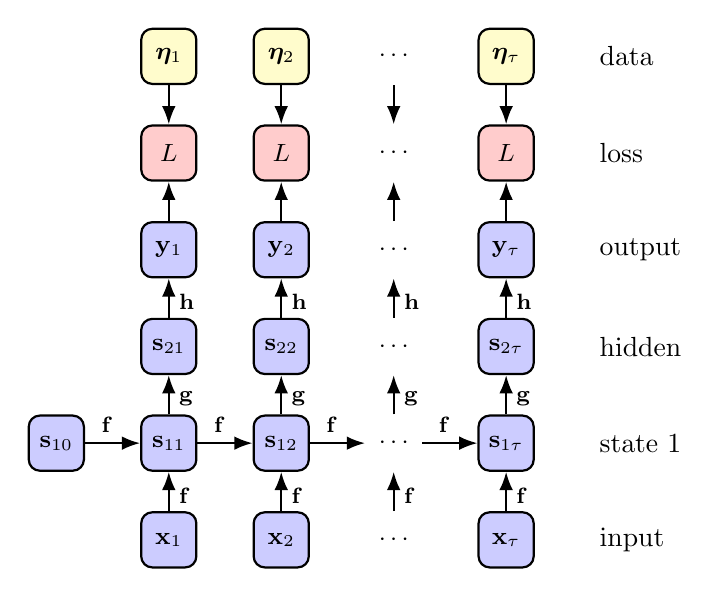
\begin{tikzpicture}[node distance=5mm, auto]
    % States.
    \node (state11) [state] {$\s_{11}$};
    \node (state10) [state, left=7mm of state11] {$\s_{10}$};
    \node (state12) [state, right=7mm of state11] {$\s_{12}$};
    \node (state13) [block, right=7mm of state12] {$\cdots$};
    \node (state14) [state, right=7mm of state13] {$\s_{1\tau}$};

    \node (state21) [state, above=of state11] {$\s_{21}$};
    \node (state22) [state, above=of state12] {$\s_{22}$};
    \node (state23) [block, above=of state13] {$\cdots$};
    \node (state24) [state, above=of state14] {$\s_{2\tau}$};


    % Inputs, outputs, losses.
    \foreach\i in {1,2} {
        \node (input\i) [state, below=of state1\i] {$\x_\i$};
        \node (output\i) [state, above=of state2\i] {$\y_\i$};
        \node (loss\i) [function, above=of output\i] {$L$};
        \node (data\i) [data, above=of loss\i] {$\ETA_\i$};
    }

    \node (input3) [block, below=of state13] {$\cdots$};
    \node (output3) [block, above=of state23] {$\cdots$};
    \node (loss3) [block, above=of output3] {$\cdots$};
    \node (data3) [block, above=of loss3] {$\cdots$};

    \node (input4) [state, below=of state14] {$\x_\tau$};
    \node (output4) [state, above=of state24] {$\y_\tau$};
    \node (loss4) [function, above=of output4] {$L$};
    \node (data4) [data, above=of loss4] {$\ETA_\tau$};

    % Labels.
    \foreach \l in {input, output, loss, data} {
        \node [right=7mm of \l4] {\l};
    }

    \node [right=7mm of state14] {state 1};
    \node [right=7mm of state24] {hidden};

    % Arrows.
    \foreach\i in {1, ..., 4} {
        \draw [path] (input\i) -- node [label, pos=0.4, right] {$\f$} (state1\i);
        \draw [path] (state1\i) -- node [label, pos=0.4, right] {$\g$} (state2\i);
        \draw [path] (state2\i) -- node [label, pos=0.4, right] {$\h$} (output\i);
        \draw [path] (output\i) -- (loss\i);
        \draw [path] (data\i) -- (loss\i);
    }

    \foreach\i/\j in {0/1, 1/2, 2/3, 3/4} {
        \draw [path] (state1\i) -- node [label, pos=0.4] {$\f$} (state1\j);
    }
\end{tikzpicture}
%%% Local Variables:
%%% mode: latex
%%% TeX-master: "../rnn"
%%% End:

    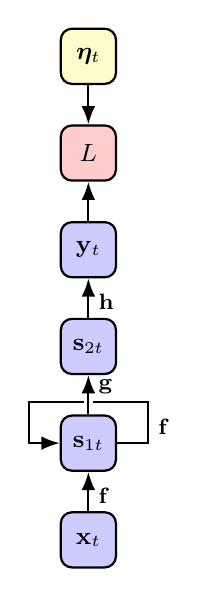
\begin{tikzpicture}[node distance=5mm, auto]
    \node (state 1) [state] {$\s_{1t}$};
    \node (state 2) [state, above=of state 1] {$\s_{2t}$};
    \node (input) [state, below=of state 1] {$\x_t$};
    \node (output) [state, above=of state 2] {$\y_t$};
    \node (loss) [function, above=of output] {$L$};
    \node (data) [data, above=of loss] {$\ETA_t$};

    \foreach \i in {1, 2} {%
        \node (skip \i) [inner sep=0.5mm, above=1mm of state \i] {};
        \node (skip \i l) [coordinate, left=7mm of skip \i] {};
        \node (skip \i r) [coordinate, right=7mm of skip \i] {};
    }

    % Arrows.
    \draw [path] (input) -- node [label, pos=0.4, right] {$\f$} (state 1);
    \draw [path] (state 1) -- node [label, pos=0.7, right] {$\g$} (state 2);
    \draw [path] (state 2) -- node [label, pos=0.4, right] {$\h$} (output);
    \draw [path] (output) -- (loss);
    \draw [path] (data) -- (loss);

    \foreach \i/\j in {1/\f} {%
        \draw [thick] (state \i) -| node [label, right, pos=0.7] {$\j$} (skip \i r) -- (skip \i);
        \draw [path] (skip \i) -- (skip \i l) |- (state \i);
    }
\end{tikzpicture}
%%% Local Variables:
%%% mode: latex
%%% TeX-master: "../rnn"
%%% End:

\end{frame}

\begin{frame}{Other deep \rnn{}s: multiple recurrent state layers \citep{GravesICASSP13}}
    \hspace{2cm}
    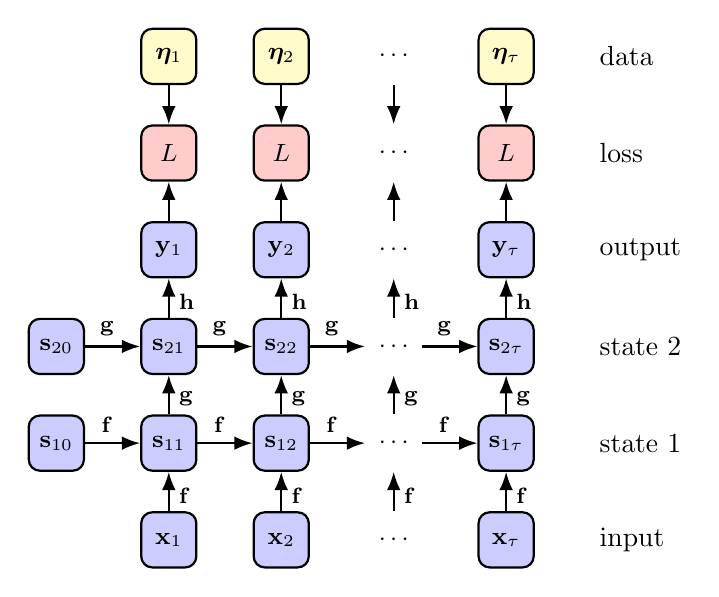
\begin{tikzpicture}[node distance=5mm, auto]
    % States.
    \node (state11) [state] {$\s_{11}$};
    \node (state10) [state, left=7mm of state11] {$\s_{10}$};
    \node (state12) [state, right=7mm of state11] {$\s_{12}$};
    \node (state13) [block, right=7mm of state12] {$\cdots$};
    \node (state14) [state, right=7mm of state13] {$\s_{1\tau}$};

    \node (state21) [state, above=of state11] {$\s_{21}$};
    \node (state20) [state, left=7mm of state21] {$\s_{20}$};
    \node (state22) [state, above=of state12] {$\s_{22}$};
    \node (state23) [block, above=of state13] {$\cdots$};
    \node (state24) [state, above=of state14] {$\s_{2\tau}$};


    % Inputs, outputs, losses.
    \foreach\i in {1,2} {
        \node (input\i) [state, below=of state1\i] {$\x_\i$};
        \node (output\i) [state, above=of state2\i] {$\y_\i$};
        \node (loss\i) [function, above=of output\i] {$L$};
        \node (data\i) [data, above=of loss\i] {$\ETA_\i$};
    }

    \node (input3) [block, below=of state13] {$\cdots$};
    \node (output3) [block, above=of state23] {$\cdots$};
    \node (loss3) [block, above=of output3] {$\cdots$};
    \node (data3) [block, above=of loss3] {$\cdots$};

    \node (input4) [state, below=of state14] {$\x_\tau$};
    \node (output4) [state, above=of state24] {$\y_\tau$};
    \node (loss4) [function, above=of output4] {$L$};
    \node (data4) [data, above=of loss4] {$\ETA_\tau$};

    % Labels.
    \foreach \l in {input, output, loss, data} {
        \node [right=7mm of \l4] {\l};
    }

    \foreach \i in {1, 2} {%
        \node [right=7mm of state\i4] {state \i};
    }

    % Arrows.
    \foreach\i in {1, ..., 4} {
        \draw [path] (input\i) -- node [label, pos=0.4, right] {$\f$} (state1\i);
        \draw [path] (state1\i) -- node [label, pos=0.4, right] {$\g$} (state2\i);
        \draw [path] (state2\i) -- node [label, pos=0.4, right] {$\h$} (output\i);
        \draw [path] (output\i) -- (loss\i);
        \draw [path] (data\i) -- (loss\i);
    }

    \foreach\i/\j in {0/1, 1/2, 2/3, 3/4} {
        \draw [path] (state1\i) -- node [label, pos=0.4] {$\f$} (state1\j);
        \draw [path] (state2\i) -- node [label, pos=0.4] {$\g$} (state2\j);
    }
\end{tikzpicture}
%%% Local Variables:
%%% mode: latex
%%% TeX-master: "../rnn"
%%% End:

    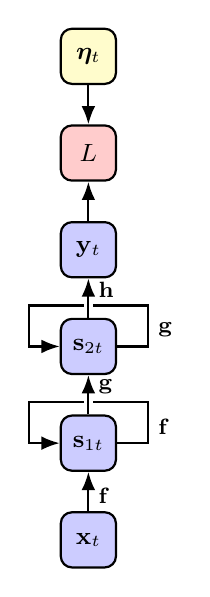
\begin{tikzpicture}[node distance=5mm, auto]
    \node (state 1) [state] {$\s_{1t}$};
    \node (state 2) [state, above=of state 1] {$\s_{2t}$};
    \node (input) [state, below=of state 1] {$\x_t$};
    \node (output) [state, above=of state 2] {$\y_t$};
    \node (loss) [function, above=of output] {$L$};
    \node (data) [data, above=of loss] {$\ETA_t$};

    \foreach \i in {1, 2} {%
        \node (skip \i) [inner sep=0.5mm, above=1mm of state \i] {};
        \node (skip \i l) [coordinate, left=7mm of skip \i] {};
        \node (skip \i r) [coordinate, right=7mm of skip \i] {};
    }

    % Arrows.
    \draw [path] (input) -- node [label, pos=0.4, right] {$\f$} (state 1);
    \draw [path] (state 1) -- node [label, pos=0.7, right] {$\g$} (state 2);
    \draw [path] (state 2) -- node [label, pos=0.7, right] {$\h$} (output);
    \draw [path] (output) -- (loss);
    \draw [path] (data) -- (loss);

    \foreach \i/\j in {1/\f, 2/\g} {%
        \draw [thick] (state \i) -| node [label, right, pos=0.7] {$\j$} (skip \i r) -- (skip \i);
        \draw [path] (skip \i) -- (skip \i l) |- (state \i);
    }
\end{tikzpicture}
%%% Local Variables:
%%% mode: latex
%%% TeX-master: "../rnn"
%%% End:

\end{frame}

\begin{frame}{Other deep \rnn{}s: deep state-to-state connections \citep{PascanuICLR14}}
    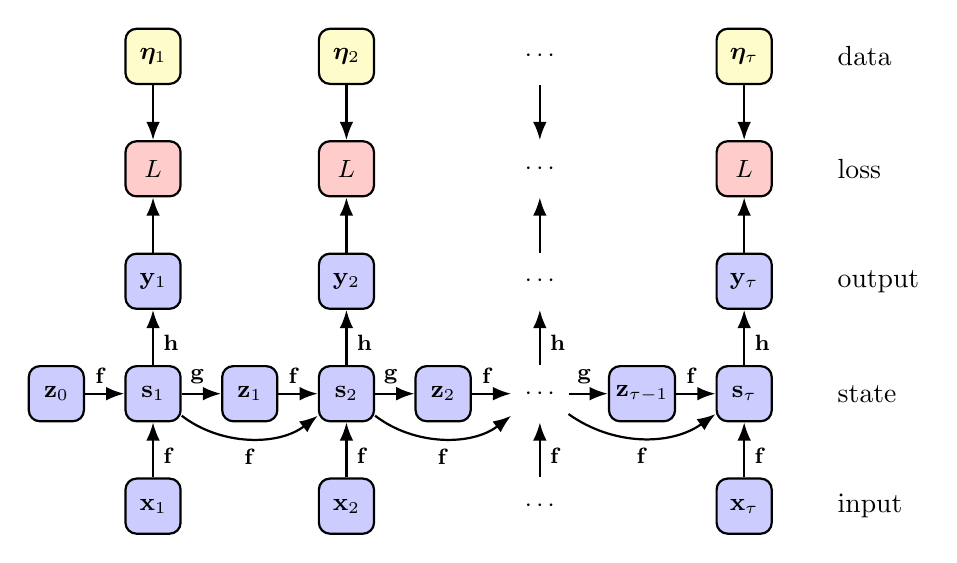
\begin{tikzpicture}[node distance=7mm, auto]
    % States.
    \node (state05) [state] {$\z_0$};
    \node (state1) [state, right=5mm of state05] {$\s_1$};
    \node (state15) [state, right=5mm of state1] {$\z_1$};
    \node (state2) [state, right=5mm of state15] {$\s_2$};
    \node (state25) [state, right=5mm of state2] {$\z_2$};
    \node (state3) [block, right=5mm of state25] {$\cdots$};
    \node (state35) [state, right=5mm of state3] {$\z_{\tau-1}$};
    \node (state4) [state, right=5mm of state35] {$\s_\tau$};

    % Inputs, outputs, losses.
    \foreach \i in {1,2} {
        \node (input\i) [state, below=of state\i] {$\x_\i$};
        \node (output\i) [state, above=of state\i] {$\y_\i$};
        \node (loss\i) [function, above=of output\i] {$L$};
        \node (data\i) [data, above=of loss\i] {$\ETA_\i$};
    }

    \node (input3) [block, below=of state3] {$\cdots$};
    \node (output3) [block, above=of state3] {$\cdots$};
    \node (loss3) [block, above=of output3] {$\cdots$};
    \node (data3) [block, above=of loss3] {$\cdots$};

    \node (input4) [state, below=of state4] {$\x_\tau$};
    \node (output4) [state, above=of state4] {$\y_\tau$};
    \node (loss4) [function, above=of output4] {$L$};
    \node (data4) [data, above=of loss4] {$\ETA_\tau$};

    % Skip connection points.
    \foreach \i in {1, ..., 3} {%
        \node (control\i1) [coordinate, below=3mm of state\i5.225] {};
        \node (control\i2) [coordinate, below=3mm of state\i5.315] {};
    }

    % Labels.
    \foreach \l in {state, input, output, loss, data} {
        \node [right=of \l4] {\l};
    }

    % Arrows.
    \foreach \i in {1, ..., 4} {
        \draw [path] (input\i) -- node [label, pos=0.4, right] {$\f$} (state\i);
        \draw [path] (state\i) -- node [label, pos=0.4, right] {$\h$} (output\i);
        \draw [path] (output\i) -- (loss\i);
        \draw [path] (data\i) -- (loss\i);
    }

    \foreach \i in {1, ..., 3} {%
        \draw [path] (state\i) -- node [label, pos=0.4] {$\g$} (state\i5);
    }

    \foreach \i in {0, ..., 3} {
        \pgfmathtruncatemacro{\j}{\i + 1}
        \draw [path] (state\i5) -- node [label, pos=0.4] {$\f$} (state\j);
    }

    % Skip connections.
    \uncover<2->{
        \foreach \i in {1, ..., 3} {
            \pgfmathtruncatemacro{\j}{\i + 1}
            \draw [path] (state\i) ..
            controls (control\i1) and (control\i2) ..
            node [label, below] {$\f$} (state\j);
        }
    }
\end{tikzpicture}
%%% Local Variables:
%%% mode: latex
%%% TeX-master: "../rnn"
%%% End:

    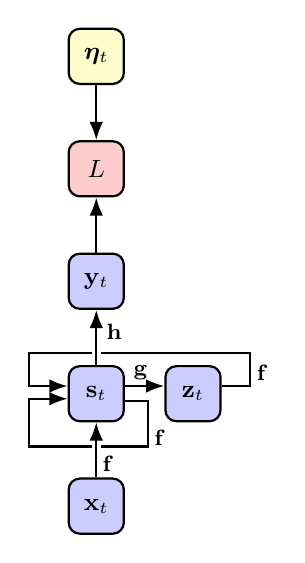
\begin{tikzpicture}[node distance=7mm, auto]
    \node (state) [state] {$\s_t$};
    \node (state 1) [state, right=5mm of state] {$\z_t$};
    \node (input) [state, below=of state] {$\x_t$};
    \node (output) [state, above=of state] {$\y_t$};
    \node (loss) [function, above=of output] {$L$};
    \node (data) [data, above=of loss] {$\ETA_t$};

    \node (skip 0) [inner sep=0.5mm, above=1mm of state] {};
    \node (skip 00) [coordinate, left=8mm of skip 0] {};
    \node (skip 01) [coordinate, right=19mm of skip 0] {};

    \node (skip 1) [inner sep=0.5mm, below=2.5mm of state] {};
    \node (skip 10) [coordinate, left=8mm of skip 1] {};
    \node (skip 11) [coordinate, right=6mm of skip 1] {};

    % Arrows.
    \draw [path] (input) --
    node [label, pos=0.25, right, xshift=-0.5mm] {$\f$}
    (state);
    \draw [path] (state) -- node [label, pos=0.6, right] {$\h$} (output);
    \draw [path] (output) -- (loss);
    \draw [path] (data) -- (loss);

    \draw [path] (state.15) --
    node [label, pos=0.4, yshift=-0.5mm] {$\g$}
    (state 1.165);
    \draw [thick] (state 1.15) -|
    node [label, right, pos=0.7, xshift=-0.5mm] {$\f$}
    (skip 01) -- (skip 0);
    \draw [path] (skip 0) -- (skip 00) |- (state.165);

    \uncover<2->{
        \draw [thick] (state.345) -|
        node [label, pos=0.9, xshift=-0.5mm] {$\f$}
        (skip 11) -- (skip 1);
        \draw [path] (skip 1) -- (skip 10) |- (state.190);
    }
\end{tikzpicture}
%%% Local Variables:
%%% mode: latex
%%% TeX-master: "../rnn"
%%% End:

\end{frame}

\begin{frame}{Odds \& ends (1/2)}
    \begin{itemize}
        \item<+-> Skip connections help prevent vanishing/exploding gradients by shortening state-to-state paths
        \item<+-> Gradient clipping helps prevent exploding gradients \citep{MikolovPhD12,PascanuICML13}
        \item<+-> Stateful \rnn{}
        \begin{itemize}[<.->]
            \item Typically, initialize cell state to $\s_0 = \zero$
            \item<+-> Stateful: set $\s_0$ to be $\s_\tau$ from the last \rnn{} invocation
            \item Used when actual sequence length $>$ RNN length: each RNN invocation extends previous one
            \item Use truncated backpropagation through time: only backprop through beginning of RNN, not beginning of sequence
        \end{itemize}
    \end{itemize}

    \centering
    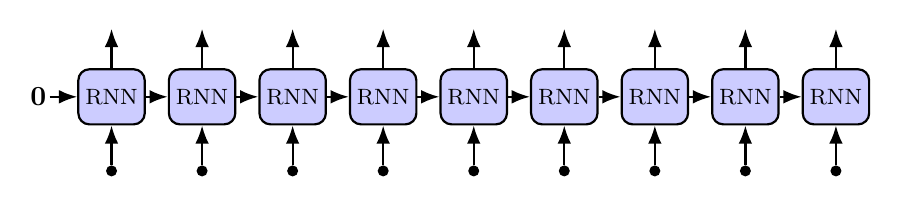
\begin{tikzpicture}[x=1.15cm, y=5mm]
    \node (input 0) [coordinate] at (0, 0) {};

    \foreach \i in {0, ..., 8} {
        \node (input \i) [fill=black, circle, minimum width=1.4mm, inner sep=0pt] at (\i, 0) {};
    }

    \uncover<2>{
        \foreach \i in {0, ..., 2} {
            \node (rnn \i) [lstm, above=5mm of input \i, font=\footnotesize] {RNN};
        }
    }

    \node (rnn -1) [left=3.5mm of rnn 0, inner sep=1pt] {$\zero$};

    \uncover<3>{
        \foreach \i in {3, ..., 5} {
            \node (rnn \i) [lstm, above=5mm of input \i, font=\footnotesize] {RNN};
        }
    }

    \uncover<4>{
        \foreach \i in {6, ..., 8} {
            \node (rnn \i) [lstm, above=5mm of input \i, font=\footnotesize] {RNN};
        }
    }

    \foreach \i in {0, ..., 8} {
        \node (output \i) [coordinate, above=5mm of rnn \i] {};
    }

    \draw [path] (rnn -1) -- (rnn 0);

    \uncover<2>{
        \draw [path] (input 0) -- (rnn 0);
        \draw [path] (rnn 0) -- (output 0);

        \foreach \i in {1, 2} {
            \pgfmathtruncatemacro{\j}{\i - 1}
            \draw [path] (input \i) -- (rnn \i);
            \draw [path] (rnn \j) -- (rnn \i);
            \draw [path] (rnn \i) -- (output \i);
        }
    }

    \uncover<3>{
        \foreach \i in {3, ..., 5} {
            \pgfmathtruncatemacro{\j}{\i - 1}
            \draw [path] (input \i) -- (rnn \i);
            \draw [path] (rnn \j) -- (rnn \i);
            \draw [path] (rnn \i) -- (output \i);
        }
    }

    \uncover<4>{
        \foreach \i in {6, ..., 8} {
            \pgfmathtruncatemacro{\j}{\i - 1}
            \draw [path] (input \i) -- (rnn \i);
            \draw [path] (rnn \j) -- (rnn \i);
            \draw [path] (rnn \i) -- (output \i);
        }
    }
\end{tikzpicture}

%%% Local Variables:
%%% mode: latex
%%% TeX-master: "../rnn"
%%% End:

\end{frame}

\begin{frame}{Odds \& ends (2/2)}
    \begin{itemize}
        \item<+-> Variable-length \rnn{}
        \begin{itemize}
            \item Beauty of \rnn{} is that length $\tau$ need not be fixed
            \item Recall silly example: variable length of speech auto $\to$ variable length sentence
            \item But static-length \rnn{}s are more computationally optimizable
        \end{itemize}
        \item<+-> Variable-length inputs/outputs
        \begin{itemize}
            \item Common approach: add \texttt{<end>} token to vocabulary; stop \rnn{} when \texttt{<end>} sampled
            \item More generally: add extra scalar output that ends \rnn{} when condition met
            \item Alternate approach: add output that predicts length $\tau$; then run for $\tau$ steps
            \begin{itemize}
                \item Important to add $\tau$ or $\tau - t$ as input to node $t$, lest sequence ends abruptly
            \end{itemize}
        \end{itemize}
    \end{itemize}
\end{frame}

%%% Local Variables:
%%% mode: latex
%%% TeX-master: "../rnn"
%%% End:

\section{Inputs \& outputs}
\subsection{}

\begin{frame}{Fixed-sized inputs}
    \begin{columns}
        \begin{column}{0.15\textwidth}
            \uncover<2->{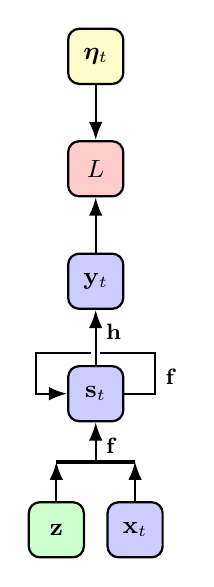
\begin{tikzpicture}[node distance=7mm, auto]
    \node (state) [state] {$\s_t$};
    \node (input) [state, below=1cm of state, xshift=5mm] {$\x_t$};
    \node (latent) [latent, below=1cm of state, xshift=-5mm] {$\z$};
    \node (output) [state, above=of state] {$\y_t$};
    \node (loss) [function, above=of output] {$L$};
    \node (data) [data, above=of loss] {$\ETA_t$};
    \node (skip) [inner sep=0.5mm, above=1mm of state] {};
    \node (skip l) [coordinate, left=7mm of skip] {};
    \node (skip r) [coordinate, right=7mm of skip] {};
    \node (above) [coordinate, below=5mm of state] {};

    % Mux.
    \foreach \n in {input, latent} {
        \node (above \n) [coordinate, above=5mm of \n] {};
        \draw [path] (\n) -- (above \n);
    }

    \draw [ultra thick] (above input) -- (above latent);

    % Arrows.
    \draw [path] (above) -- node [label, pos=0.4, right] {$\f$} (state);
    \draw [path] (state) -- node [label, pos=0.6, right] {$\h$} (output);
    \draw [path] (output) -- (loss);
    \draw [path] (data) -- (loss);
    \draw [thick] (state) -| node [label, right, pos=0.7] {$\f$} (skip r) -- (skip);
    \draw [path] (skip) -- (skip l) |- (state);
\end{tikzpicture}
%%% Local Variables:
%%% mode: latex
%%% TeX-master: "../rnn"
%%% End:
}
        \end{column}
        \begin{column}{0.41\textwidth}
            In some RNN applications, need to feed in constant \emph{fixed-size} $\z \in \Reals^l$
            \begin{itemize}
                \item<+-> I.e., not a sequence
                \item $\z$ may be contextual information, or a latent vector
                \item Input sequence $\x_t$ might not even exist
                \item E.g., latent-to-sequence decoder
            \end{itemize}
            \uncover<+->{Common approaches}
            \begin{itemize}
                \item<.-> Left: append $\z$ to \emph{every} input $\x_t$
                \item<+-> Right: set initial state $\s_0 = \z$
                \item<.-> Combination of both
            \end{itemize}
        \end{column}
        \begin{column}{0.44\textwidth}
            \uncover<3->{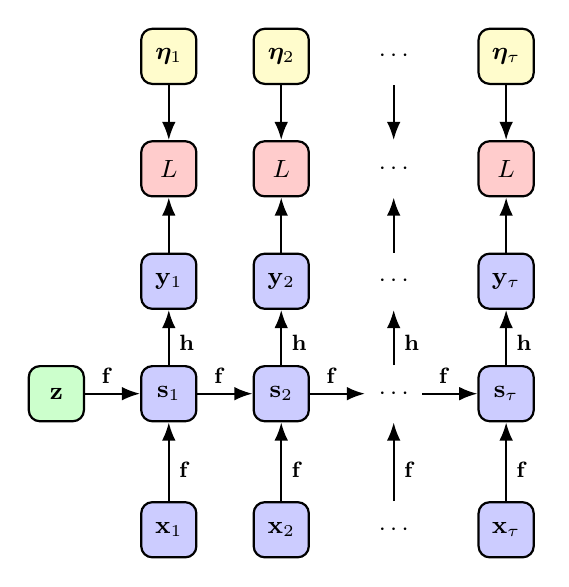
\begin{tikzpicture}[node distance=7mm, auto]
    % States.
    \node (state0) [latent] {$\z$};
    \node (state1) [state, right=of state0] {$\s_1$};
    \node (state2) [state, right=of state1] {$\s_2$};
    \node (state3) [block, right=of state2] {$\cdots$};
    \node (state4) [state, right=of state3] {$\s_\tau$};

    % Inputs, outputs, losses.
    \foreach\i in {1, 2} {
        \node (input\i) [state, below=1 cm of state\i] {$\x_\i$};
        \node (output\i) [state, above=of state\i] {$\y_\i$};
        \node (loss\i) [function, above=of output\i] {$L$};
        \node (data\i) [data, above=of loss\i] {$\ETA_\i$};
    }

    \node (input3) [block, below=1cm of state3] {$\cdots$};
    \node (output3) [block, above=of state3] {$\cdots$};
    \node (loss3) [block, above=of output3] {$\cdots$};
    \node (data3) [block, above=of loss3] {$\cdots$};

    \node (input4) [state, below=1cm of state4] {$\x_\tau$};
    \node (output4) [state, above=of state4] {$\y_\tau$};
    \node (loss4) [function, above=of output4] {$L$};
    \node (data4) [data, above=of loss4] {$\ETA_\tau$};

    % Arrows.
    \foreach\i in {1, ..., 4} {
        \draw [path] (input\i) -- node [label, pos=0.4, right] {$\f$} (state\i);
        \draw [path] (state\i) -- node [label, pos=0.4, right] {$\h$} (output\i);
        \draw [path] (output\i) -- (loss\i);
        \draw [path] (data\i) -- (loss\i);
    }

    \foreach\i/\j in {0/1, 1/2, 2/3, 3/4} {
        \draw [path] (state\i) -- node [label, pos=0.4] {$\f$} (state\j);
    }
\end{tikzpicture}
%%% Local Variables:
%%% mode: latex
%%% TeX-master: "../rnn"
%%% End:
}
            \vspace{-4mm}
        \end{column}
    \end{columns}
\end{frame}

\begin{frame}{Fixed-size outputs}
    \begin{columns}
        \begin{column}{0.37\textwidth}
            \uncover<2->{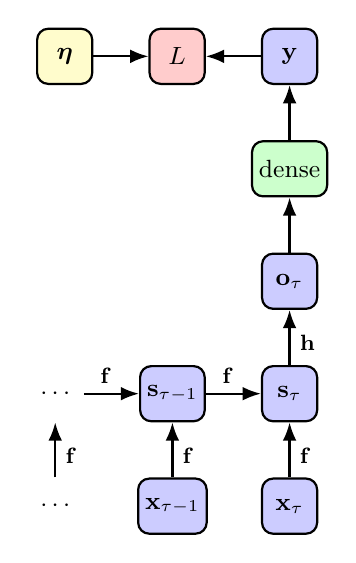
\begin{tikzpicture}[node distance=7mm, auto]
    % States.
    \node (state2) [block] {$\cdots$};
    \node (state3) [state, right=of state2] {$\s_{\tau-1}$};
    \node (state4) [state, right=of state3] {$\s_\tau$};

    % Inputs.
    \node (input2) [block, below=of state2] {$\cdots$};

    \foreach\i/\j in {3/-1, 4/} {
        \node (input\i) [state, below=of state\i] {$\x_{\tau\j}$};
    }

    % Outputs, etc.
    \node (rnn output) [state, above=of state4] {$\o_\tau$};
    \node (dense) [dense, above=of rnn output] {dense};
    \node (dense output) [state, above=of dense] {$\y$};
    \node (loss) [function, left=of dense output] {$L$};
    \node (data) [data, left=of loss] {$\ETA$};

    % Arrows.
    \foreach\i in {2, ..., 4} {
        \draw [path] (input\i) -- node [label, pos=0.4, right] {$\f$} (state\i);
    }

    \foreach\i/\j in {2/3, 3/4} {
        \draw [path] (state\i) -- node [label, pos=0.4] {$\f$} (state\j);
    }

    \draw [path] (state4) -- node [label, pos=0.4, right] {$\h$} (rnn output);
    \draw [path] (rnn output) -- (dense);
    \draw [path] (dense) -- (dense output);
    \draw [path] (dense output) -- (loss);
    \draw [path] (data) -- (loss);
\end{tikzpicture}
%%% Local Variables:
%%% mode: latex
%%% TeX-master: "../rnn"
%%% End:
}
        \end{column}
        \begin{column}{0.63\textwidth}
            In some RNN applications, need a \emph{fixed-size} output $\y \in \Reals^p$
            \begin{itemize}
                \item<+-> I.e., not a sequence
                \item $\y$ may be classification of a sequence
                \item $\y$ may be a latent vector, e.g., sequence encoder
            \end{itemize}
            \uncover<+->{Common approach}
            \begin{itemize}[<.->]
                \item Ignore all RNN outputs $\o_t$ except the last
                \item Feed $\o_\tau$ to dense layer(s)
                \item Final dense layer has width $p$ and output $\y$
            \end{itemize}
            \uncover<+->{Justification}
            \begin{itemize}[<.->]
                \item Final output $\o_\tau$ encodes information about \emph{entire} input $\x_1, \ldots, \x_\tau$
                \item Dense layers reshape dimensions and provide extra processing
            \end{itemize}
        \end{column}
    \end{columns}
\end{frame}

\begin{frame}{Encoder--decoder sequence-to-sequence models, figure}
    \vspace{5mm}
    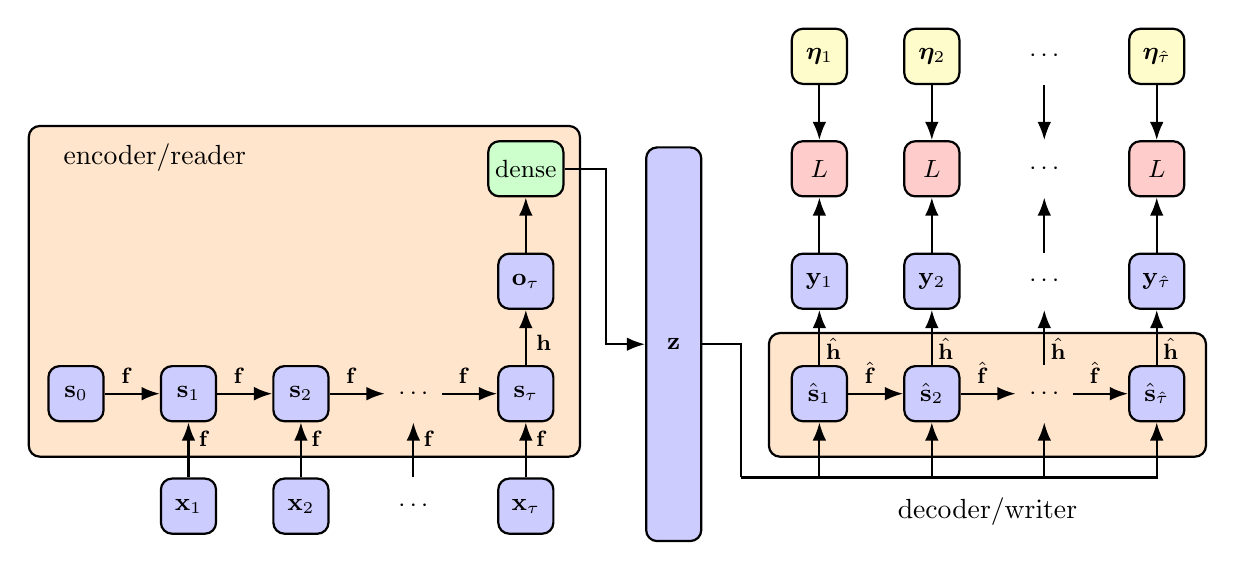
\begin{tikzpicture}[node distance=7mm, auto]
    % Encoder.

    \draw [cell, fill=orange!20] (-0.6, -0.8) rectangle (6.4, 3.4);

    % States.
    \node (e state0) [state] {$\s_0$};
    \node (e state1) [state, right=of e state0] {$\s_1$};
    \node (e state2) [state, right=of e state1] {$\s_2$};
    \node (e state3) [block, right=of e state2] {$\cdots$};
    \node (e state4) [state, right=of e state3] {$\s_\tau$};

    % Inputs.
    \node (e input1) [state, below=of e state1] {$\x_1$};
    \node (e input2) [state, below=of e state2] {$\x_2$};
    \node (e input3) [block, below=of e state3] {$\cdots$};
    \node (e input4) [state, below=of e state4] {$\x_\tau$};

    % Outputs, etc.
    \node (rnn output) [state, above=of e state4] {$\o_\tau$};
    \node (dense) [dense, above=of rnn output] {dense};
    \node (latent) [state, right=1.15cm of rnn output, minimum height=5cm, yshift=-8mm] {$\z$};
    \node (latent input) [coordinate, left=5mm of latent] {};

    % Arrows.
    \foreach\i in {1, ..., 4} {
        \draw [path] (e input\i) -- node [label, pos=0.7, right] {$\f$} (e state\i);
    }

    \foreach\i/\j in {0/1, 1/2, 2/3, 3/4} {
        \draw [path] (e state\i) -- node [label, pos=0.4] {$\f$} (e state\j);
    }

    \draw [path] (e state4) -- node [label, pos=0.4, right] {$\h$} (rnn output);
    \draw [path] (rnn output) -- (dense);
    \draw [path] (dense) -| (latent input) -- (latent);

    % Decoder.
    \uncover<2->{
        \draw [cell, fill=orange!20] (8.8, -0.8) rectangle (14.35, 0.77);

        % States.
        \node (d state1) [state, right=of e state4, xshift=2.3cm] {$\hat{\s}_1$};
        \node (d state2) [state, right=of d state1] {$\hat{\s}_2$};
        \node (d state3) [block, right=of d state2] {$\cdots$};
        \node (d state4) [state, right=of d state3] {$\hat{\s}_{\hat{\tau}}$};

        % Inputs.
        \node (d input1) [coordinate, below=of d state1] {};
        \node (d input0) [coordinate, left=1cm of d input1] {};

        % Outputs & losses.
        \foreach\i in {1,2} {
            \node (output\i) [state, above=of d state\i] {$\y_\i$};
            \node (loss\i) [function, above=of output\i] {$L$};
            \node (data\i) [data, above=of loss\i] {$\ETA_\i$};
        }
        g
        \node (output3) [block, above=of d state3] {$\cdots$};
        \node (loss3) [block, above=of output3] {$\cdots$};
        \node (data3) [block, above=of loss3] {$\cdots$};

        \node (output4) [state, above=of d state4] {$\y_{\hat{\tau}}$};
        \node (loss4) [function, above=of output4] {$L$};
        \node (data4) [data, above=of loss4] {$\ETA_{\hat{\tau}}$};

        % Arrows.
        \draw [thick] (latent) -| (d input0);

        \foreach\i in {1, ..., 4} {
            \draw [path] (d input0) -| (d state\i);
            \draw [path] (d state\i) -- node [label, pos=0.3, right, xshift=-0.5mm] {$\hat{\h}$} (output\i);
            \draw [path] (output\i) -- (loss\i);
            \draw [path] (data\i) -- (loss\i);
        }

        \foreach\i/\j in {1/2, 2/3, 3/4} {
            \draw [path] (d state\i) -- node [label, pos=0.4] {$\hat{\f}$} (d state\j);
        }
    }
    % Labels.

    \node at (1, 3) {encoder/reader};
    \uncover<2->{\node at (11.575, -1.5) {decoder/writer};}
\end{tikzpicture}
%%% Local Variables:
%%% mode: latex
%%% TeX-master: "../rnn"
%%% End:

    \vspace{-2.5mm}

    \begin{textblock}{9.5}(1,2)
        If inputs $\x_1, \dots, \x_\tau$ and outputs $\y_1, \dots, \y_{\hat{\tau}}$ have different/variable lengths, \alert{encode} inputs to latent vector $\z \in \Reals^l$\uncover<2->{, and \alert{decode} $\z$ to outputs}
    \end{textblock}
\end{frame}

% To do: explain attention mechanism.
\begin{frame}{Encoder--decoder sequence-to-sequence models, notes}
    \begin{itemize}
        \item Introduced by \citet{ChoEMNLP14}, \citet{Sutskever14}
        \item Many ways to connect encoder and decoder
        \begin{itemize}
            \item Simplest: $\hat{\s}_1 = \s_\tau$; forces $\dim(\s_t) = \dim(\hat{\s}_t)$
            \item As shown: use dense layer on encoder output $\o_\tau$; allows $\dim(\z) \ne \dim(\s_t)$
            \item As aforementioned: can feed $\z$ as input to every input (as shown), use $\hat{\s}_1 = \z$ (forces $\dim(\z) = \dim(\hat{\s}_{\hat{t}})$), or both
        \end{itemize}
        \pause
        \item Problem: difficult to encode all of $\x_1, \dots, \x_\tau$ in single vector $\z$ extracted from $\s_\tau$, especially for large $\tau$
        \item Solution: attention mechanism \citep{BahdanauICLR15}
        \begin{itemize}
            \item Encoder hidden states $\s_1, \dots, \s_\tau$ are stored
            \item At each $\hat{t}$ in the decoder, weighted average of $\s_1, \dots, \s_\tau$ forms context vector $\c_{\hat{t}}$
            \item Weights are based on how well $\s_t$ aligns with $\hat{\s}_{\hat{t}}$
            \item Context vector $\c_{\hat{t}}$ fed into decoder
        \end{itemize}
    \end{itemize}
\end{frame}

\begin{frame}{Embeddings}
    \begin{itemize}
        \item When classifying by one-hot encoding, all $c$ classes are $\sqrt{2}$ apart in $L^2$ distance
        \item One-hot is fine for small $c$, but dim-$\tilde{c}$ embeddings ($\tilde{c} \ll c$) generally do better for large $c$
        \item E.g., \texttt{sheep} should have smaller distance to \texttt{ewe} or \texttt{goat} than to \texttt{quasar} or \texttt{supersonic}
        \item Embeddings can be pre-trained, or simultaneously trained with RNN
        \item Note: not at all unique to RNNs
    \end{itemize}

    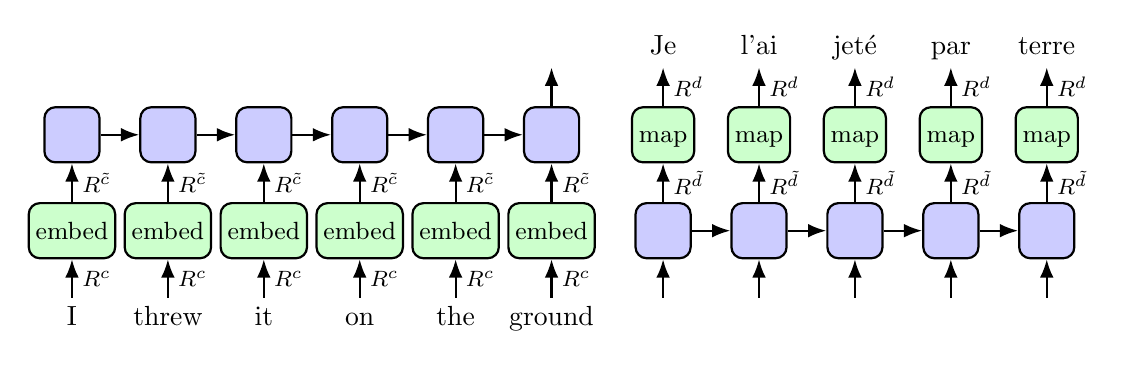
\begin{tikzpicture}[node distance=4.9mm, auto]
    % Embeddings.
    \node (e rnn 0) [lstm] {\rnn};

    \foreach \i in {0, ..., 4} {
        \pgfmathtruncatemacro{\j}{\i + 1}
        \node (e rnn \j) [lstm, right=of e rnn \i] {\rnn};
    }

    \foreach \i in {0, ..., 5} {
        \node (embed \i) [dense, below=of e rnn \i] {embed};
        \node (e output \i) [coordinate, above=of e rnn \i] {};
    }

    \node (e input 0) [word, below=of embed 0] {I};
    \node (e input 1) [word, below=of embed 1] {threw};
    \node (e input 2) [word, below=of embed 2] {it};
    \node (e input 3) [word, below=of embed 3] {on};
    \node (e input 4) [word, below=of embed 4] {the};
    \node (e input 5) [word, below=of embed 5] {ground};

    \node (e output) [coordinate, above=of e rnn 5] {};

    \foreach \i in {0, ..., 5} {
        \draw [path] (e input \i) -- node [label, right] {$\Reals^c$} (embed \i);
        \draw [path] (embed \i) -- node [label, right] {$\Reals^{\tilde{c}}$} (e rnn \i);
    }

    \foreach \i in {0, ..., 4} {
        \pgfmathtruncatemacro{\j}{\i + 1}
        \draw [path] (e rnn \i) -- (e rnn \j);
    }

    \draw [path] (e rnn 5) -- (e output);

    % Projections.
    \node (f rnn 0) [lstm, right=of embed 5] {\rnn};

    \foreach \i in {0, ..., 3} {
        \pgfmathtruncatemacro{\j}{\i + 1}
        \node (f rnn \j) [lstm, right=of f rnn \i] {\rnn};
    }

    \foreach \i in {0, ..., 4} {
        \node (f input \i) [coordinate, below=of f rnn \i] {};
        \node (project \i) [word, dense, above=of f rnn \i] {map};
    }

    \node (f output 0) [word, above=of project 0] {Je};
    \node (f output 1) [word, above=of project 1] {l'ai};
    \node (f output 2) [word, above=of project 2] {jet\'e};
    \node (f output 3) [word, above=of project 3] {par};
    \node (f output 4) [word, above=of project 4] {terre};

    \foreach \i in {0, ..., 4} {
        \draw [path] (f input \i) -- (f rnn \i);
        \draw [path] (f rnn \i) -- node [label, right] {$\Reals^{\tilde{d}}$} (project \i);
        \draw [path] (project \i) -- node [label, right] {$\Reals^d$} (f output \i);
    }

    \foreach \i in {0, ..., 3} {
        \pgfmathtruncatemacro{\j}{\i + 1}
        \draw [path] (f rnn \i) -- (f rnn \j);
    }
\end{tikzpicture}

%%% Local Variables:
%%% mode: latex
%%% TeX-master: "../rnn"
%%% End:

\end{frame}

%%% Local Variables:
%%% mode: latex
%%% TeX-master: "../rnn"
%%% End:

\section{Alternate architectures}
\subsection{}

% To do: explain HMM.
\begin{frame}{RNNs and Hidden Markov Models}
    \begin{columns}
        \begin{column}{0.46\textwidth}
            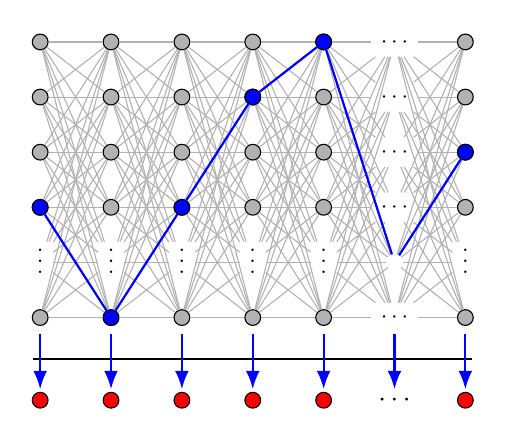
\begin{tikzpicture}[x=9mm, y=7mm]
    % All States.
    \foreach \i in {1, ..., 5, 7} {
        \foreach \j in {1, 3, 4, ..., 6} {
            \node (\i\j) [hmm] at (\i, \j) {};
        }

        \node (\i2) at (\i, 2) [label] {\vvdots};
    }

    \foreach \j in {1, 3, 4, ..., 6} {
        \node (6\j) at (6, \j) [label] {$\cdots$};
    }

    \node (62) [circle, minimum width=2mm, inner sep=0pt] at (6, 2) {};

    % Traversed states.
    \node (state 13) [hmm, fill=blue] at (1, 3) {};
    \node (state 21) [hmm, fill=blue] at (2, 1) {};
    \node (state 33) [hmm, fill=blue] at (3, 3) {};
    \node (state 45) [hmm, fill=blue] at (4, 5) {};
    \node (state 56) [hmm, fill=blue] at (5, 6) {};
    \node (state 74) [hmm, fill=blue] at (7, 4) {};

    % All connections.
    \foreach \i in {1, ..., 6} {
        \pgfmathtruncatemacro{\j}{\i + 1}

        \foreach \k in {1, ..., 6} {
            \foreach \l in {1, ..., 6} {
                \draw [black!30] (\i\k) -- (\j\l);
            }
        }
    }

    % Traversed connections.
    \draw [blue, thick] (state 13) -- (state 21);
    \draw [blue, thick] (state 21) -- (state 33);
    \draw [blue, thick] (state 33) -- (state 45);
    \draw [blue, thick] (state 45) -- (state 56);
    \draw [blue, thick] (state 56) -- (62);
    \draw [blue, thick] (62) -- (state 74);

    % Outputs.
    \draw [thick] (0.9, 0.25) -- (7.1, 0.25);

    \foreach \i in {1, ..., 5, 7} {
        \node [hmm, fill=red] at (\i, -0.5) {};
    }

    \node at (6, -0.5) {$\cdots$};

    \foreach \i in {1, ..., 7} {
        \draw [path, blue] (\i, 0.7) -- (\i, -0.3);
    }
\end{tikzpicture}

%%% Local Variables:
%%% mode: latex
%%% TeX-master: "../rnn"
%%% End:

        \end{column}
        \begin{column}{0.54\textwidth}
            \begin{itemize}
                \item<+-> RNNs are deterministic, HMMs are stochastic
                \item<.-> But posterior probabilities of states and outputs of HMMs are deterministic
            \end{itemize}
            \begin{block}{}<+->
                An HMM, when viewed in terms of probabilities, is a special case of an RNN
            \end{block}
            \begin{itemize}[<.->]
                \item HMM transition probabilities analogous to RNN weights
                \item<+-> Why do traditional RNNs and HMMs excel at different tasks?
                \item What about a task makes each work well?
                \item What can each do well that the other cannot?
            \end{itemize}
        \end{column}
    \end{columns}
\end{frame}

\begin{frame}{1-D convolutional neural networks}
    Sequences analogous to 1-D space
    \begin{itemize}
        \item<+-> Physics/engineering analogy: time analogous to 1-D space
        \item Ordinary differential equation methods translate between the two
    \end{itemize}
    \uncover<+->{Can use 1-D CNNs to process sequences}

    \begin{center}
        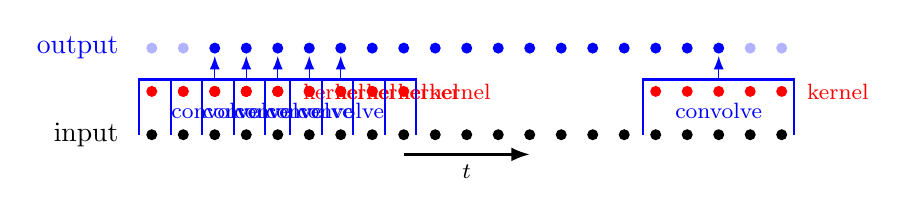
\begin{tikzpicture}[x=4mm, y=5mm]
    \node (input 0) [coordinate] at (0, 0) {};
    \node (output 0) [coordinate] at (0, 2.2) {};

    \uncover<.->{
        \foreach \i in {0, ..., 20} {
            \fill [black] (\i, 0) circle (0.7mm);
        }

        \node [align=right, left=3mm of input 0] {input};
        \draw [path] (8, -0.5) -- node [label, below] {$t$} (12, -0.5);
    }

    \visible<3->{
        \foreach \i in {0, 1} {
            \fill[blue!30] (\i, 2.2) circle (0.7mm);
        }

        \node [align=right, left=3mm of output 0, blue] {output};
    }

    \foreach \i in {2, ..., 6} {
        \visible<+|handout:0>{
            \node [label, blue] at (\i, 0.6) {convolve};

            \foreach \j in {-2, ..., 2} {
                \fill [red] (\i+\j, 1.1) circle (0.7mm);
            }

            \draw [thick, blue] (\i-2.4, 0) -- (\i-2.4, 1.4) -- (\i+2.4, 1.4) -- (\i+2.4, 0);
            \node at (\i+2, 1.1) [label, anchor=west, xshift=2mm, red] {kernel};
            \draw [-Latex, blue] (\i, 1.4) -- (\i, 2);
        }

        \visible<.->{\fill [blue] (\i, 2.2) circle (0.7mm);}
    }

    \visible<+->{
        \def\i{18}
        \node [label, blue] at (\i, 0.6) {convolve};

        \foreach \j in {-2, ..., 2} {
            \fill [red] (\i+\j, 1.1) circle (0.7mm);
        }

        \draw [thick, blue] (\i-2.4, 0) -- (\i-2.4, 1.4) -- (\i+2.4, 1.4) -- (\i+2.4, 0);
        \node at (\i+2, 1.1) [label, anchor=west, xshift=2mm, red] {kernel};
        \draw [-Latex, blue] (\i, 1.4) -- (\i, 2);
        \fill [blue] (\i, 2.2) circle (0.7mm);

        \foreach \i in {7, ..., 17} {
            \fill [blue] (\i, 2.2) circle (0.7mm);
        }

        \foreach \i in {19, 20} {
            \fill [blue!30] (\i, 2.2) circle (0.7mm);
        }
    }
\end{tikzpicture}

%%% Local Variables:
%%% mode: latex
%%% TeX-master: "../rnn"
%%% End:


        \uncover<+->{
            \begin{tabular}{c|c}
                RNN & CNN \\
                \hline
                $\y_t$ depends on $\s_0, \dots, \s_t$, also $\s_{t+1}, \dots, \s_\tau$ if desired &
                $\y_t$ depends on $\s_{t-\delta}, \dots, \s_{t+\delta}$ \\
                generally non-parallelizable across $t$ & parallelizable across $t$ \\
            \end{tabular}
        }
    \end{center}

    \uncover<.->{
        RNNs generally stronger than 1-D CNNs for sequences;
        RNN cell state intuitively helpful
    }
\end{frame}

\begin{frame}{Recursive neural networks}
    \begin{columns}
        \begin{column}{0.61\textwidth}
            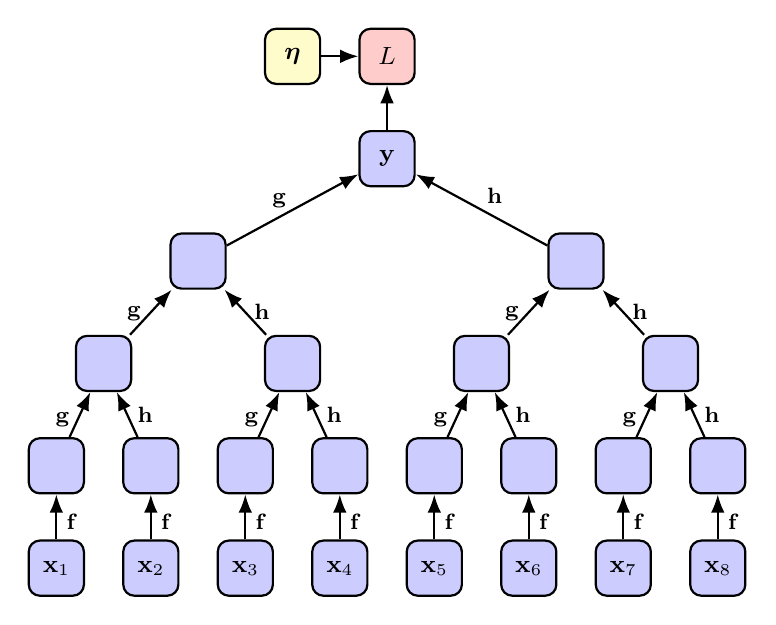
\begin{tikzpicture}[x=1.2cm, y=1.3cm, auto]
    \foreach \i in {1, ..., 8} {
        \node (input \i) [state] at (\i, 0) {$\x_\i$};
        \node (state 1\i) [state] at (\i, 1) {};
        \draw [path] (input \i) -- node [label, right, pos=0.4] {$\f$} (state 1\i);
    }

    \node (state 21) [state] at (1.5, 2) {};
    \node (state 22) [state] at (3.5, 2) {};
    \node (state 23) [state] at (5.5, 2) {};
    \node (state 24) [state] at (7.5, 2) {};

    \node (state 31) [state] at (2.5, 3) {};
    \node (state 32) [state] at (6.5, 3) {};

    \node (output) [state] at (4.5, 4) {$\y$};
    \node (loss) [function] at (4.5, 5) {$L$};
    \node (data) [data] at (3.5, 5) {$\ETA$};

    \foreach \j in {1, ..., 4} {
        \pgfmathtruncatemacro{\i}{2 * \j - 1}
        \draw [path] (state 1\i) -- node [word, label, left] {$\g$} (state 2\j);
    }

    \foreach \j in {1, ..., 4} {
        \pgfmathtruncatemacro{\i}{2 * \j}
        \draw [path] (state 1\i) -- node [label, right] {$\h$} (state 2\j);
    }

    \foreach \i/\j in {1/1, 3/2} {
        \draw [path] (state 2\i) -- node [word, label, above, pos=0.1] {$\g$} (state 3\j);
    }

    \foreach \i/\j in {2/1, 4/2} {
        \draw [path] (state 2\i) -- node [label, above, pos=0.1] {$\h$} (state 3\j);
    }

    \draw [path] (state 31) -- node [word, label, above, pos=0.4] {$\g$} (output);
    \draw [path] (state 32) -- node [word, label, above, pos=0.4] {$\h$} (output);

    \draw [path] (output) -- (loss);
    \draw [path] (data) -- (loss);
\end{tikzpicture}

%%% Local Variables:
%%% mode: latex
%%% TeX-master: "../rnn"
%%% End:

        \end{column}
        \begin{column}{0.39\textwidth}
            \begin{itemize}
                \item Introduced by \citet{PollackAI90}
                \item Advantage: longest connection $\approx \log_2 \tau$, rather than $\tau$
                \item Tree structure can be static or data-dependent
            \end{itemize}
        \end{column}
    \end{columns}
\end{frame}

%%% Local Variables:
%%% mode: latex
%%% TeX-master: "../rnn"
%%% End:

\section{Examples}
\subsection{}

%%% Local Variables:
%%% mode: latex
%%% TeX-master: "../rnn"
%%% End:

\section{Conclusion}
\subsection{}

\begin{frame}{Conclusion}
    \begin{itemize}
        \item \rnn{}s are a powerful way to model sequences
        \item Flexible: inputs \& outputs can be fixed-length sequences, variable-length sequences, fixed-size vectors, etc.
        \item \lstm{}s and \gru{}s are the best architectures today
        \item $\# \text{params} \sim (\text{state size})^2$,
        $\# \text{ops} \sim \text{length} \cdot (\text{state size})^2$
        \begin{itemize}
            \item Generally non-parallelizable in time
            \item Watch out for long \rnn{}s and large state sizes
        \end{itemize}
        \item Many ways to make deep; stacking is most common
    \end{itemize}
    % Advertise software tutorial
\end{frame}

%%% Local Variables:
%%% mode: latex
%%% TeX-master: "../rnn"
%%% End:

\footnotesize

\begin{frame}[allowframebreaks]{References}
    \bibliography{rnn}
\end{frame}

%%% Local Variables:
%%% mode: latex
%%% TeX-master: "../rnn"
%%% End:


\end{document}

%%% Local Variables:
%%% mode: latex
%%% TeX-master: t
%%% End:
